\documentclass[twoside]{book}

% Packages required by doxygen
\usepackage{fixltx2e}
\usepackage{calc}
\usepackage{doxygen}
\usepackage[export]{adjustbox} % also loads graphicx
\usepackage{graphicx}
\usepackage[utf8]{inputenc}
\usepackage{makeidx}
\usepackage{multicol}
\usepackage{multirow}
\PassOptionsToPackage{warn}{textcomp}
\usepackage{textcomp}
\usepackage[nointegrals]{wasysym}
\usepackage[table]{xcolor}

% NLS support packages
\usepackage[french]{babel}
\NoAutoSpaceBeforeFDP

% Font selection
\usepackage[T1]{fontenc}
\usepackage[scaled=.90]{helvet}
\usepackage{courier}
\usepackage{amssymb}
\usepackage{sectsty}
\renewcommand{\familydefault}{\sfdefault}
\allsectionsfont{%
  \fontseries{bc}\selectfont%
  \color{darkgray}%
}
\renewcommand{\DoxyLabelFont}{%
  \fontseries{bc}\selectfont%
  \color{darkgray}%
}
\newcommand{\+}{\discretionary{\mbox{\scriptsize$\hookleftarrow$}}{}{}}

% Page & text layout
\usepackage{geometry}
\geometry{%
  a4paper,%
  top=2.5cm,%
  bottom=2.5cm,%
  left=2.5cm,%
  right=2.5cm%
}
\tolerance=750
\hfuzz=15pt
\hbadness=750
\setlength{\emergencystretch}{15pt}
\setlength{\parindent}{0cm}
\setlength{\parskip}{3ex plus 2ex minus 2ex}
\makeatletter
\renewcommand{\paragraph}{%
  \@startsection{paragraph}{4}{0ex}{-1.0ex}{1.0ex}{%
    \normalfont\normalsize\bfseries\SS@parafont%
  }%
}
\renewcommand{\subparagraph}{%
  \@startsection{subparagraph}{5}{0ex}{-1.0ex}{1.0ex}{%
    \normalfont\normalsize\bfseries\SS@subparafont%
  }%
}
\makeatother

% Headers & footers
\usepackage{fancyhdr}
\pagestyle{fancyplain}
\fancyhead[LE]{\fancyplain{}{\bfseries\thepage}}
\fancyhead[CE]{\fancyplain{}{}}
\fancyhead[RE]{\fancyplain{}{\bfseries\leftmark}}
\fancyhead[LO]{\fancyplain{}{\bfseries\rightmark}}
\fancyhead[CO]{\fancyplain{}{}}
\fancyhead[RO]{\fancyplain{}{\bfseries\thepage}}
\fancyfoot[LE]{\fancyplain{}{}}
\fancyfoot[CE]{\fancyplain{}{}}
\fancyfoot[RE]{\fancyplain{}{\bfseries\scriptsize Généré par Doxygen }}
\fancyfoot[LO]{\fancyplain{}{\bfseries\scriptsize Généré par Doxygen }}
\fancyfoot[CO]{\fancyplain{}{}}
\fancyfoot[RO]{\fancyplain{}{}}
\renewcommand{\footrulewidth}{0.4pt}
\renewcommand{\chaptermark}[1]{%
  \markboth{#1}{}%
}
\renewcommand{\sectionmark}[1]{%
  \markright{\thesection\ #1}%
}

% Indices & bibliography
\usepackage{natbib}
\usepackage[titles]{tocloft}
\setcounter{tocdepth}{3}
\setcounter{secnumdepth}{5}
\makeindex

% Hyperlinks (required, but should be loaded last)
\usepackage{ifpdf}
\ifpdf
  \usepackage[pdftex,pagebackref=true]{hyperref}
\else
  \usepackage[ps2pdf,pagebackref=true]{hyperref}
\fi
\hypersetup{%
  colorlinks=true,%
  linkcolor=blue,%
  citecolor=blue,%
  unicode%
}

% Custom commands
\newcommand{\clearemptydoublepage}{%
  \newpage{\pagestyle{empty}\cleardoublepage}%
}

\usepackage{caption}
\captionsetup{labelsep=space,justification=centering,font={bf},singlelinecheck=off,skip=4pt,position=top}

%===== C O N T E N T S =====

\begin{document}

% Titlepage & ToC
\hypersetup{pageanchor=false,
             bookmarksnumbered=true,
             pdfencoding=unicode
            }
\pagenumbering{alph}
\begin{titlepage}
\vspace*{7cm}
\begin{center}%
{\Large Iryal.\+io }\\
\vspace*{1cm}
{\large Généré par Doxygen 1.8.14}\\
\end{center}
\end{titlepage}
\clearemptydoublepage
\pagenumbering{roman}
\tableofcontents
\clearemptydoublepage
\pagenumbering{arabic}
\hypersetup{pageanchor=true}

%--- Begin generated contents ---
\chapter{Liste des bogues}
\label{bug}
\Hypertarget{bug}

\begin{DoxyRefList}
\item[\label{bug__bug000001}%
\Hypertarget{bug__bug000001}%
Membre \mbox{\hyperlink{class_mur_a63a7560c521670716cd90c3599abcd71}{Mur\+:\+:collision}} (\mbox{\hyperlink{class_cercle}{Cercle}} \&) const]des fois la double collision ne marche pas. la plupart des cas c\textquotesingle{}est se voit quand la distance entre deux mur est plus grand que le rayon et inférieur 2$\ast$r.
\end{DoxyRefList}
\chapter{Index des espaces de nommage}
\section{Liste des espaces de nommage}
Liste de tous les espaces de nommage documentés avec une brève description\+:\begin{DoxyCompactList}
\item\contentsline{section}{\mbox{\hyperlink{namespacesocklib}{socklib}} \\*Espace de nom général }{\pageref{namespacesocklib}}{}
\end{DoxyCompactList}

\chapter{Index hiérarchique}
\section{Hiérarchie des classes}
Cette liste d\textquotesingle{}héritage est classée approximativement par ordre alphabétique \+:\begin{DoxyCompactList}
\item \contentsline{section}{Cercle}{\pageref{class_cercle}}{}
\item \contentsline{section}{console}{\pageref{classconsole}}{}
\item \contentsline{section}{Couleur}{\pageref{class_couleur}}{}
\item \contentsline{section}{Fenetre}{\pageref{class_fenetre}}{}
\item \contentsline{section}{Fenetre\+S\+F\+ML}{\pageref{class_fenetre_s_f_m_l}}{}
\item \contentsline{section}{Image}{\pageref{class_image}}{}
\item \contentsline{section}{Iryal\+\_\+io}{\pageref{class_iryal__io}}{}
\item \contentsline{section}{Jeu}{\pageref{class_jeu}}{}
\item \contentsline{section}{Joueur}{\pageref{class_joueur}}{}
\item \contentsline{section}{Menu}{\pageref{class_menu}}{}
\item \contentsline{section}{Rectangle}{\pageref{class_rectangle}}{}
\begin{DoxyCompactList}
\item \contentsline{section}{Camera}{\pageref{class_camera}}{}
\item \contentsline{section}{Case}{\pageref{class_case}}{}
\item \contentsline{section}{Mur}{\pageref{class_mur}}{}
\item \contentsline{section}{Terrain}{\pageref{class_terrain}}{}
\end{DoxyCompactList}
\item \contentsline{section}{Reseau}{\pageref{class_reseau}}{}
\item \contentsline{section}{Tab\+Dyn$<$ T $>$}{\pageref{class_tab_dyn}}{}
\end{DoxyCompactList}

\chapter{Index des classes}
\section{Liste des classes}
Liste des classes, structures, unions et interfaces avec une brève description \+:\begin{DoxyCompactList}
\item\contentsline{section}{\mbox{\hyperlink{class_camera}{Camera}} \\*Hérite du class \mbox{\hyperlink{class_rectangle}{Rectangle}} cette classe permet de afficher que les objet sur la camera }{\pageref{class_camera}}{}
\item\contentsline{section}{\mbox{\hyperlink{class_case}{Case}} }{\pageref{class_case}}{}
\item\contentsline{section}{\mbox{\hyperlink{class_cercle}{Cercle}} }{\pageref{class_cercle}}{}
\item\contentsline{section}{\mbox{\hyperlink{classconsole}{console}} }{\pageref{classconsole}}{}
\item\contentsline{section}{\mbox{\hyperlink{class_couleur}{Couleur}} }{\pageref{class_couleur}}{}
\item\contentsline{section}{\mbox{\hyperlink{class_fenetre}{Fenetre}} }{\pageref{class_fenetre}}{}
\item\contentsline{section}{\mbox{\hyperlink{class_fenetre_s_f_m_l}{Fenetre\+S\+F\+ML}} }{\pageref{class_fenetre_s_f_m_l}}{}
\item\contentsline{section}{\mbox{\hyperlink{class_image}{Image}} \\*La classe contoent le lien vers une image dans une chaine de tableau }{\pageref{class_image}}{}
\item\contentsline{section}{\mbox{\hyperlink{class_iryal__io}{Iryal\+\_\+io}} }{\pageref{class_iryal__io}}{}
\item\contentsline{section}{\mbox{\hyperlink{class_jeu}{Jeu}} }{\pageref{class_jeu}}{}
\item\contentsline{section}{\mbox{\hyperlink{class_joueur}{Joueur}} }{\pageref{class_joueur}}{}
\item\contentsline{section}{\mbox{\hyperlink{class_menu}{Menu}} }{\pageref{class_menu}}{}
\item\contentsline{section}{\mbox{\hyperlink{class_mur}{Mur}} }{\pageref{class_mur}}{}
\item\contentsline{section}{\mbox{\hyperlink{class_rectangle}{Rectangle}} }{\pageref{class_rectangle}}{}
\item\contentsline{section}{\mbox{\hyperlink{class_reseau}{Reseau}} }{\pageref{class_reseau}}{}
\item\contentsline{section}{\mbox{\hyperlink{class_tab_dyn}{Tab\+Dyn$<$ T $>$}} }{\pageref{class_tab_dyn}}{}
\item\contentsline{section}{\mbox{\hyperlink{class_terrain}{Terrain}} \\*Un terrain possède une position, un largeur et une hauteur }{\pageref{class_terrain}}{}
\end{DoxyCompactList}

\chapter{Index des fichiers}
\section{Liste des fichiers}
Liste de tous les fichiers documentés avec une brève description \+:\begin{DoxyCompactList}
\item\contentsline{section}{src/base/{\bfseries Case.\+h} }{\pageref{_case_8h}}{}
\item\contentsline{section}{src/base/{\bfseries Cercle.\+h} }{\pageref{_cercle_8h}}{}
\item\contentsline{section}{src/base/{\bfseries Couleur.\+h} }{\pageref{_couleur_8h}}{}
\item\contentsline{section}{src/base/{\bfseries Image.\+h} }{\pageref{_image_8h}}{}
\item\contentsline{section}{src/base/{\bfseries Rectangle.\+h} }{\pageref{_rectangle_8h}}{}
\item\contentsline{section}{src/base/{\bfseries Reseau.\+h} }{\pageref{_reseau_8h}}{}
\item\contentsline{section}{src/base/\mbox{\hyperlink{socklib_8hpp}{socklib.\+hpp}} \\*Fichier contenant les fonctions de créations de socket et les fonctions de gestion d\textquotesingle{}erreur }{\pageref{socklib_8hpp}}{}
\item\contentsline{section}{src/base/{\bfseries Tab\+Dyn.\+h} }{\pageref{_tab_dyn_8h}}{}
\item\contentsline{section}{src/base/{\bfseries tools.\+h} }{\pageref{tools_8h}}{}
\item\contentsline{section}{src/base/{\bfseries Vec2.\+h} }{\pageref{_vec2_8h}}{}
\item\contentsline{section}{src/core/{\bfseries Camera.\+h} }{\pageref{_camera_8h}}{}
\item\contentsline{section}{src/core/{\bfseries Iryal\+\_\+io.\+h} }{\pageref{_iryal__io_8h}}{}
\item\contentsline{section}{src/core/{\bfseries Jeu.\+h} }{\pageref{_jeu_8h}}{}
\item\contentsline{section}{src/core/{\bfseries Joueur.\+h} }{\pageref{_joueur_8h}}{}
\item\contentsline{section}{src/core/{\bfseries Menu.\+h} }{\pageref{_menu_8h}}{}
\item\contentsline{section}{src/core/{\bfseries Mur.\+h} }{\pageref{_mur_8h}}{}
\item\contentsline{section}{src/core/{\bfseries Terrain.\+h} }{\pageref{_terrain_8h}}{}
\item\contentsline{section}{src/sdl/{\bfseries Fenetre.\+h} }{\pageref{_fenetre_8h}}{}
\item\contentsline{section}{src/sdlnet/{\bfseries Net\+S\+D\+L.\+h} }{\pageref{_net_s_d_l_8h}}{}
\item\contentsline{section}{src/sfml/{\bfseries Fenetre\+S\+F\+M\+L.\+h} }{\pageref{_fenetre_s_f_m_l_8h}}{}
\item\contentsline{section}{src/txt/{\bfseries console.\+h} }{\pageref{console_8h}}{}
\end{DoxyCompactList}

\chapter{Documentation des espaces de nommage}
\hypertarget{namespacesocklib}{}\section{Référence de l\textquotesingle{}espace de nommage socklib}
\label{namespacesocklib}\index{socklib@{socklib}}


espace de nom général  


\subsection*{Fonctions}
\begin{DoxyCompactItemize}
\item 
void \mbox{\hyperlink{namespacesocklib_aec23e1a0b60ca039283516d2305f799e}{\+\_\+\+\_\+error\+\_\+}} (const char $\ast$file, const int ligne, const std\+::string \&msg, bool cond, int errnum, bool exception)
\begin{DoxyCompactList}\small\item\em fonction générique de la gestion d\textquotesingle{}erreur \end{DoxyCompactList}\item 
int \mbox{\hyperlink{namespacesocklib_af229dcfe18deb451a8163a02ea5a3b06}{Cree\+Socket\+Serveur}} (const std\+::string \&port)
\begin{DoxyCompactList}\small\item\em Cree une socket d\textquotesingle{}attente pour le serveur sur le port \textquotesingle{}\textquotesingle{}port\textquotesingle{}\textquotesingle{}. \end{DoxyCompactList}\item 
int \mbox{\hyperlink{namespacesocklib_a426a4d6e2fbcf559659e88607f0473f7}{Cree\+Socket\+Client}} (const std\+::string \&server, const std\+::string \&port)
\begin{DoxyCompactList}\small\item\em Crée une socket de client en se connectant à un serveur. \end{DoxyCompactList}\item 
int \mbox{\hyperlink{namespacesocklib_a56cdbced316496706a18df3f6a62d28f}{Accept\+Connexion}} (int s)
\begin{DoxyCompactList}\small\item\em Accepte un nouveau client. \end{DoxyCompactList}\end{DoxyCompactItemize}


\subsection{Description détaillée}
espace de nom général 

\subsection{Documentation des fonctions}
\mbox{\Hypertarget{namespacesocklib_aec23e1a0b60ca039283516d2305f799e}\label{namespacesocklib_aec23e1a0b60ca039283516d2305f799e}} 
\index{socklib@{socklib}!\+\_\+\+\_\+error\+\_\+@{\+\_\+\+\_\+error\+\_\+}}
\index{\+\_\+\+\_\+error\+\_\+@{\+\_\+\+\_\+error\+\_\+}!socklib@{socklib}}
\subsubsection{\texorpdfstring{\+\_\+\+\_\+error\+\_\+()}{\_\_error\_()}}
{\footnotesize\ttfamily void socklib\+::\+\_\+\+\_\+error\+\_\+ (\begin{DoxyParamCaption}\item[{const char $\ast$}]{file,  }\item[{const int}]{ligne,  }\item[{const std\+::string \&}]{msg,  }\item[{bool}]{cond,  }\item[{int}]{errnum,  }\item[{bool}]{exception }\end{DoxyParamCaption})}



fonction générique de la gestion d\textquotesingle{}erreur 


\begin{DoxyParams}{Paramètres}
{\em file,ligne} & \+: le nom et la ligne du fichier où a lieu l\textquotesingle{}erreur \\
\hline
{\em msg} & \+: le message à afficher en cas d\textquotesingle{}erreur \\
\hline
{\em cond} & \+: la condition (l\textquotesingle{}erreure est déclanchée si elle est vraie) \\
\hline
{\em errnum} & \+: code d\textquotesingle{}erreur système \\
\hline
{\em exception} & \+: si vrai envoie une exception en cas d\textquotesingle{}erreur, sinon, c\textquotesingle{}est just un warning \\
\hline
\end{DoxyParams}
\mbox{\Hypertarget{namespacesocklib_a56cdbced316496706a18df3f6a62d28f}\label{namespacesocklib_a56cdbced316496706a18df3f6a62d28f}} 
\index{socklib@{socklib}!Accept\+Connexion@{Accept\+Connexion}}
\index{Accept\+Connexion@{Accept\+Connexion}!socklib@{socklib}}
\subsubsection{\texorpdfstring{Accept\+Connexion()}{AcceptConnexion()}}
{\footnotesize\ttfamily int socklib\+::\+Accept\+Connexion (\begin{DoxyParamCaption}\item[{int}]{s }\end{DoxyParamCaption})}



Accepte un nouveau client. 


\begin{DoxyParams}{Paramètres}
{\em s} & \+: la socket d\textquotesingle{}attente du serveur \\
\hline
\end{DoxyParams}
\begin{DoxyReturn}{Renvoie}
la socket de discution 
\end{DoxyReturn}

\begin{DoxyExceptions}{Exceptions}
{\em une} & système error s\textquotesingle{}il y a un problème \\
\hline
\end{DoxyExceptions}
\mbox{\Hypertarget{namespacesocklib_a426a4d6e2fbcf559659e88607f0473f7}\label{namespacesocklib_a426a4d6e2fbcf559659e88607f0473f7}} 
\index{socklib@{socklib}!Cree\+Socket\+Client@{Cree\+Socket\+Client}}
\index{Cree\+Socket\+Client@{Cree\+Socket\+Client}!socklib@{socklib}}
\subsubsection{\texorpdfstring{Cree\+Socket\+Client()}{CreeSocketClient()}}
{\footnotesize\ttfamily int socklib\+::\+Cree\+Socket\+Client (\begin{DoxyParamCaption}\item[{const std\+::string \&}]{server,  }\item[{const std\+::string \&}]{port }\end{DoxyParamCaption})}



Crée une socket de client en se connectant à un serveur. 


\begin{DoxyParams}{Paramètres}
{\em server,port} & \+: le serveur et le port à contacter. \\
\hline
\end{DoxyParams}
\begin{DoxyReturn}{Renvoie}
la socket de discution 
\end{DoxyReturn}

\begin{DoxyExceptions}{Exceptions}
{\em une} & system\+\_\+error s\textquotesingle{}il y a un souci à la création ou une runtime\+\_\+error si le serveur ne peut pas être contacté \\
\hline
\end{DoxyExceptions}
\mbox{\Hypertarget{namespacesocklib_af229dcfe18deb451a8163a02ea5a3b06}\label{namespacesocklib_af229dcfe18deb451a8163a02ea5a3b06}} 
\index{socklib@{socklib}!Cree\+Socket\+Serveur@{Cree\+Socket\+Serveur}}
\index{Cree\+Socket\+Serveur@{Cree\+Socket\+Serveur}!socklib@{socklib}}
\subsubsection{\texorpdfstring{Cree\+Socket\+Serveur()}{CreeSocketServeur()}}
{\footnotesize\ttfamily int socklib\+::\+Cree\+Socket\+Serveur (\begin{DoxyParamCaption}\item[{const std\+::string \&}]{port }\end{DoxyParamCaption})}



Cree une socket d\textquotesingle{}attente pour le serveur sur le port \textquotesingle{}\textquotesingle{}port\textquotesingle{}\textquotesingle{}. 


\begin{DoxyParams}{Paramètres}
{\em port} & \+: le port utilisé \\
\hline
\end{DoxyParams}
\begin{DoxyReturn}{Renvoie}
la socket d\textquotesingle{}attente 
\end{DoxyReturn}

\begin{DoxyExceptions}{Exceptions}
{\em une} & system\+\_\+error s\textquotesingle{}il y a un soucis à la création ou une runtime\+\_\+error si le port est occupé ou ne peux pas être pris\\
\hline
\end{DoxyExceptions}
En cas d\textquotesingle{}erreur, un message explicatif est affiché sur la sortie d\textquotesingle{}erreur standart 
\chapter{Documentation des classes}
\hypertarget{class_camera}{}\section{Référence de la classe Camera}
\label{class_camera}\index{Camera@{Camera}}


hérite du class \mbox{\hyperlink{class_rectangle}{Rectangle}} cette classe permet de afficher que les objet sur la camera  




{\ttfamily \#include $<$Camera.\+h$>$}

Graphe d\textquotesingle{}héritage de Camera\+:\begin{figure}[H]
\begin{center}
\leavevmode
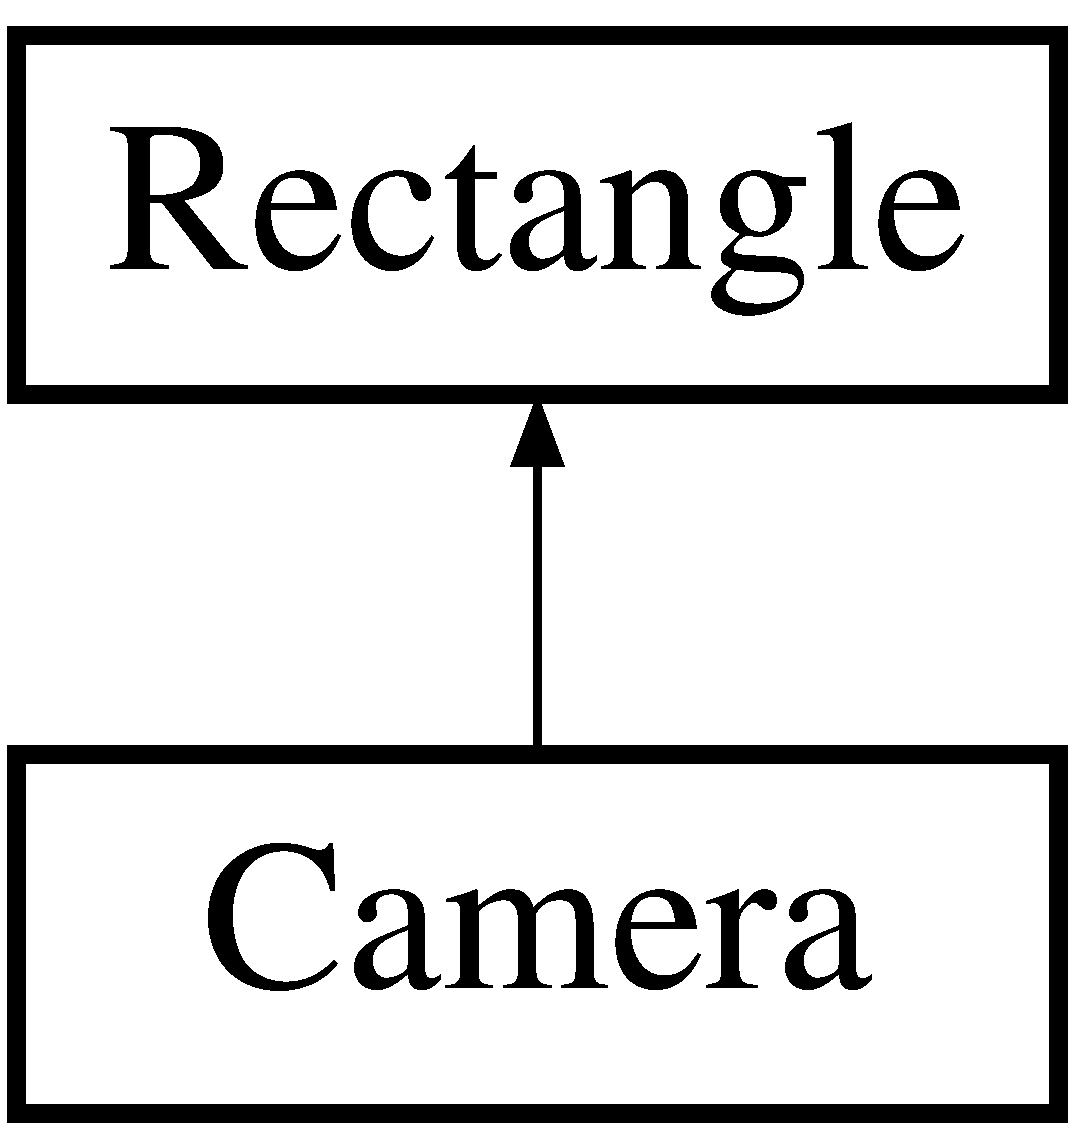
\includegraphics[height=2.000000cm]{class_camera}
\end{center}
\end{figure}
\subsection*{Fonctions membres publiques}
\begin{DoxyCompactItemize}
\item 
\mbox{\hyperlink{class_camera_ab01f0ff58d8ebd0ffbe27f62a9a9e3ac}{Camera}} (const Vec2 \&\+\_\+pos\+Min=Vec2(0, 0), unsigned int w=1, unsigned int h=1)
\item 
\mbox{\Hypertarget{class_camera_a9afa00681d1ad6e1c27e1a57f2f9fa3b}\label{class_camera_a9afa00681d1ad6e1c27e1a57f2f9fa3b}} 
{\bfseries Camera} (const \mbox{\hyperlink{class_rectangle}{Rectangle}} \&rec, Vec2 $\ast$c)
\item 
\mbox{\Hypertarget{class_camera_a6bc12c73b564c99186eb085e23ba733c}\label{class_camera_a6bc12c73b564c99186eb085e23ba733c}} 
Vec2 $\ast$ {\bfseries get\+Cam\+Cercle} ()
\item 
\mbox{\Hypertarget{class_camera_a6f7f884d3b0765cdbbce3edce865f15f}\label{class_camera_a6f7f884d3b0765cdbbce3edce865f15f}} 
Vec2 {\bfseries get\+Cam\+Pos} () const
\item 
\mbox{\Hypertarget{class_camera_a23e1db806a30ed408267108b30b030f4}\label{class_camera_a23e1db806a30ed408267108b30b030f4}} 
Vec2 \& {\bfseries get\+Pos\+Ref} ()
\item 
\mbox{\Hypertarget{class_camera_a5d2e17beaf1533caf8726b576c32ec94}\label{class_camera_a5d2e17beaf1533caf8726b576c32ec94}} 
bool {\bfseries est\+Dans\+La\+Camera} (const \mbox{\hyperlink{class_cercle}{Cercle}} \&) const
\item 
\mbox{\Hypertarget{class_camera_a2ee4df62243f38013fdfbb5aa08282d7}\label{class_camera_a2ee4df62243f38013fdfbb5aa08282d7}} 
bool {\bfseries est\+Dans\+La\+Camera} (const \mbox{\hyperlink{class_rectangle}{Rectangle}} \&) const
\item 
\mbox{\Hypertarget{class_camera_a8f888f5b620bd332c88bd49dfaaa1574}\label{class_camera_a8f888f5b620bd332c88bd49dfaaa1574}} 
void \mbox{\hyperlink{class_camera_a8f888f5b620bd332c88bd49dfaaa1574}{set\+Pos}} (Vec2 $\ast$)
\begin{DoxyCompactList}\small\item\em prends un pointeur comme la posiotion de camera on va l\textquotesingle{}utiliser pour mettre l\textquotesingle{}addresse de la position d\textquotesingle{}un cercle \end{DoxyCompactList}\item 
\mbox{\Hypertarget{class_camera_a2c0a2712a6f8cbe29a9f4ede68bf828f}\label{class_camera_a2c0a2712a6f8cbe29a9f4ede68bf828f}} 
void {\bfseries reste\+Dans\+Le\+Terrain} (const \mbox{\hyperlink{class_terrain}{Terrain}} \&)
\end{DoxyCompactItemize}
\subsection*{Attributs protégés}
\begin{DoxyCompactItemize}
\item 
\mbox{\Hypertarget{class_camera_a78d509eb873c55a2f530c7a2db318359}\label{class_camera_a78d509eb873c55a2f530c7a2db318359}} 
Vec2 $\ast$ {\bfseries Cam\+Cercle}
\end{DoxyCompactItemize}


\subsection{Description détaillée}
hérite du class \mbox{\hyperlink{class_rectangle}{Rectangle}} cette classe permet de afficher que les objet sur la camera 

\subsection{Documentation des constructeurs et destructeur}
\mbox{\Hypertarget{class_camera_ab01f0ff58d8ebd0ffbe27f62a9a9e3ac}\label{class_camera_ab01f0ff58d8ebd0ffbe27f62a9a9e3ac}} 
\index{Camera@{Camera}!Camera@{Camera}}
\index{Camera@{Camera}!Camera@{Camera}}
\subsubsection{\texorpdfstring{Camera()}{Camera()}}
{\footnotesize\ttfamily Camera\+::\+Camera (\begin{DoxyParamCaption}\item[{const Vec2 \&}]{\+\_\+pos\+Min = {\ttfamily Vec2(0,0)},  }\item[{unsigned int}]{w = {\ttfamily 1},  }\item[{unsigned int}]{h = {\ttfamily 1} }\end{DoxyParamCaption})\hspace{0.3cm}{\ttfamily [inline]}}

une camera avec la position pos\+Min, largeur et hauteur w et h en utilisant le constructeur du \mbox{\hyperlink{class_rectangle}{Rectangle}} 

La documentation de cette classe a été générée à partir des fichiers suivants \+:\begin{DoxyCompactItemize}
\item 
src/core/Camera.\+h\item 
src/core/Camera.\+cpp\end{DoxyCompactItemize}

\hypertarget{class_case}{}\section{Référence de la classe Case}
\label{class_case}\index{Case@{Case}}
Graphe d\textquotesingle{}héritage de Case\+:\begin{figure}[H]
\begin{center}
\leavevmode
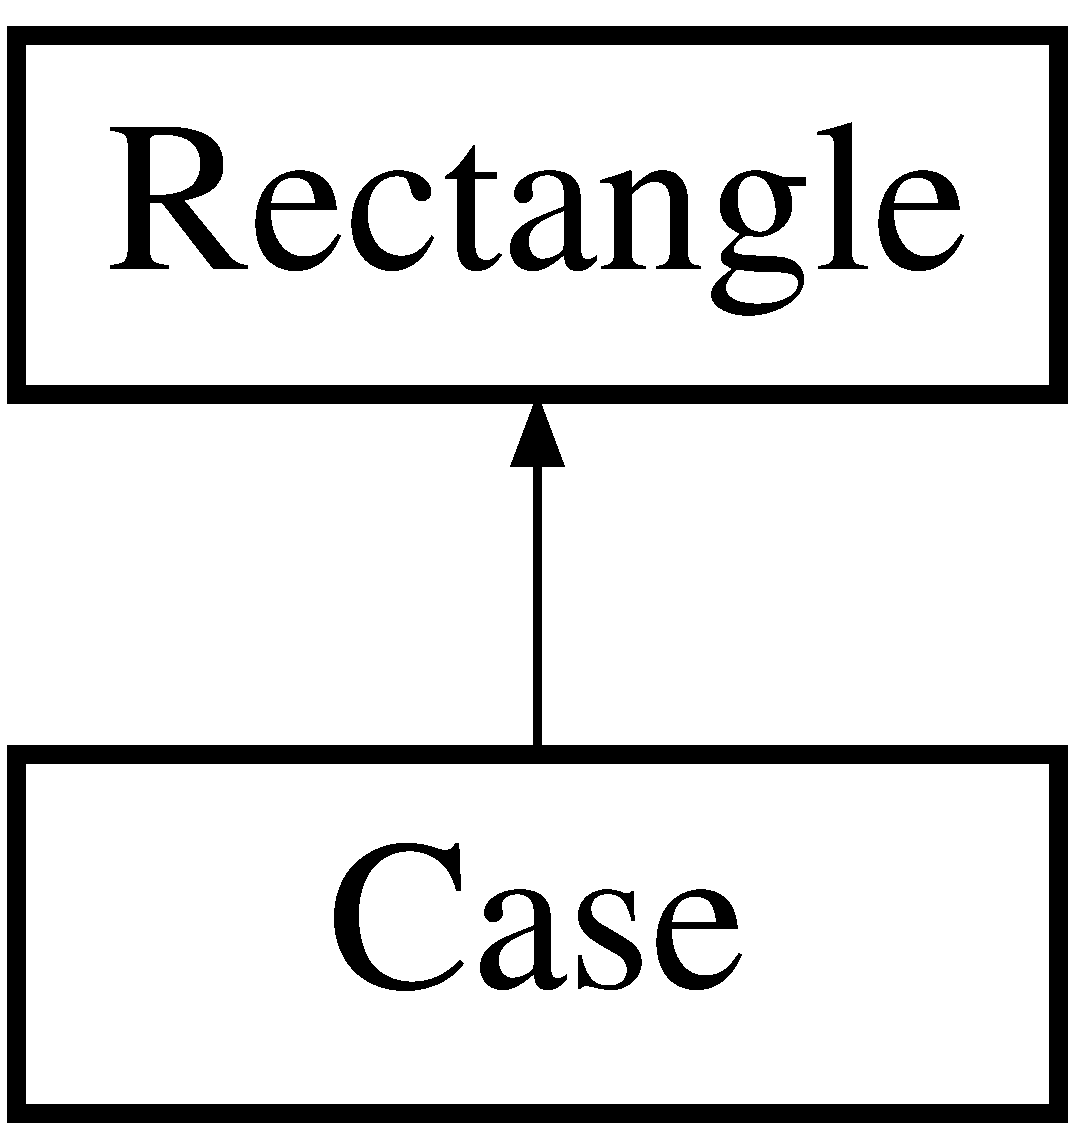
\includegraphics[height=2.000000cm]{class_case}
\end{center}
\end{figure}
\subsection*{Fonctions membres publiques}
\begin{DoxyCompactItemize}
\item 
\mbox{\Hypertarget{class_case_a459fed689a33e6389ff5f6b5620fbb1e}\label{class_case_a459fed689a33e6389ff5f6b5620fbb1e}} 
\mbox{\hyperlink{class_case_a459fed689a33e6389ff5f6b5620fbb1e}{Case}} (const Vec2 \&\+\_\+pos\+Min=Vec2(0, 0), unsigned int w=1, unsigned int h=1)
\begin{DoxyCompactList}\small\item\em constructeur pas copie initié. \end{DoxyCompactList}\item 
\mbox{\Hypertarget{class_case_acfc98a7ba6e29a1c5287834783422be8}\label{class_case_acfc98a7ba6e29a1c5287834783422be8}} 
\mbox{\hyperlink{class_case_acfc98a7ba6e29a1c5287834783422be8}{Case}} (const Vec2 \&\+\_\+pos\+Min, unsigned int w, unsigned int h, const std\+::string \&s, const etat e=jeu\+Libre)
\begin{DoxyCompactList}\small\item\em constructeur par default. \end{DoxyCompactList}\item 
\mbox{\Hypertarget{class_case_a152012a9d0be1aff1d0ca89eb784d67f}\label{class_case_a152012a9d0be1aff1d0ca89eb784d67f}} 
std\+::string {\bfseries get\+Contenu} () const
\item 
\mbox{\Hypertarget{class_case_a4f7b7781abc608b880c308728a0d8901}\label{class_case_a4f7b7781abc608b880c308728a0d8901}} 
void {\bfseries set\+Contenu} (const std\+::string \&)
\item 
\mbox{\Hypertarget{class_case_ab22ba706f90de0fac85858156d47d36d}\label{class_case_ab22ba706f90de0fac85858156d47d36d}} 
bool \mbox{\hyperlink{class_case_ab22ba706f90de0fac85858156d47d36d}{pressed}} (const Vec2 \&) const
\begin{DoxyCompactList}\small\item\em Retourne si la case est appouyyé. \end{DoxyCompactList}\item 
\mbox{\Hypertarget{class_case_ae8b2df78f80afdcdfe529ad25859cff9}\label{class_case_ae8b2df78f80afdcdfe529ad25859cff9}} 
etat \mbox{\hyperlink{class_case_ae8b2df78f80afdcdfe529ad25859cff9}{get\+\_\+etat}} () const
\begin{DoxyCompactList}\small\item\em retourne l\textquotesingle{}etat courant de la case \end{DoxyCompactList}\end{DoxyCompactItemize}
\subsection*{Attributs protégés}
\begin{DoxyCompactItemize}
\item 
\mbox{\Hypertarget{class_case_af0979bafd87649acb864af1400e80495}\label{class_case_af0979bafd87649acb864af1400e80495}} 
etat {\bfseries etat\+\_\+to\+\_\+return}
\item 
\mbox{\Hypertarget{class_case_a8a875eb6aa07f2440a534b7ac8f23ad7}\label{class_case_a8a875eb6aa07f2440a534b7ac8f23ad7}} 
std\+::string {\bfseries contenu}
\end{DoxyCompactItemize}


La documentation de cette classe a été générée à partir des fichiers suivants \+:\begin{DoxyCompactItemize}
\item 
src/base/Case.\+h\item 
src/base/Case.\+cpp\end{DoxyCompactItemize}

\hypertarget{class_cercle}{}\section{Référence de la classe Cercle}
\label{class_cercle}\index{Cercle@{Cercle}}
\subsection*{Fonctions membres publiques}
\begin{DoxyCompactItemize}
\item 
\mbox{\Hypertarget{class_cercle_a372f6c395207e159d750a4dd9d32ffba}\label{class_cercle_a372f6c395207e159d750a4dd9d32ffba}} 
\mbox{\hyperlink{class_cercle_a372f6c395207e159d750a4dd9d32ffba}{Cercle}} (unsigned int \+\_\+r=0, const Vec2 \&pos=Vec2(0, 0), const Vec2 \&\+\_\+vitesse=Vec2(0, 0))
\begin{DoxyCompactList}\small\item\em deux constructeurs par default et par copie. \end{DoxyCompactList}\item 
\mbox{\Hypertarget{class_cercle_a264c7e3272b98fe7e9846fc75fd18171}\label{class_cercle_a264c7e3272b98fe7e9846fc75fd18171}} 
{\bfseries Cercle} (float x, float y, float r)
\item 
\mbox{\Hypertarget{class_cercle_afde23d1a195aba93d89d7f5eb39c929b}\label{class_cercle_afde23d1a195aba93d89d7f5eb39c929b}} 
{\bfseries Cercle} (const \mbox{\hyperlink{class_cercle}{Cercle}} \&c)
\item 
\mbox{\Hypertarget{class_cercle_a09b99ae93d7f76990cb0249d843d2f64}\label{class_cercle_a09b99ae93d7f76990cb0249d843d2f64}} 
void {\bfseries set\+Pos\+Vec2} (float x, float y)
\item 
\mbox{\Hypertarget{class_cercle_a3c85ccf0f1d79cb0824f1bac0cb6ffd8}\label{class_cercle_a3c85ccf0f1d79cb0824f1bac0cb6ffd8}} 
float {\bfseries get\+Acc} () const
\item 
\mbox{\Hypertarget{class_cercle_a3874d00fe210def896576d30cd19baf6}\label{class_cercle_a3874d00fe210def896576d30cd19baf6}} 
Vec2 \& {\bfseries get\+Vitesse} ()
\item 
\mbox{\Hypertarget{class_cercle_a8d2427e6a2b1c610d4df4db25ea463c0}\label{class_cercle_a8d2427e6a2b1c610d4df4db25ea463c0}} 
float \mbox{\hyperlink{class_cercle_a8d2427e6a2b1c610d4df4db25ea463c0}{get\+Rayon}} () const
\begin{DoxyCompactList}\small\item\em retourne le rayon du cercle \end{DoxyCompactList}\item 
void \mbox{\hyperlink{class_cercle_aa8a8df2a669f39962bbaac2da474e401}{set\+Rayon}} (float)
\item 
\mbox{\Hypertarget{class_cercle_abc75c79032c4669d3bd30b9d504ee001}\label{class_cercle_abc75c79032c4669d3bd30b9d504ee001}} 
float \mbox{\hyperlink{class_cercle_abc75c79032c4669d3bd30b9d504ee001}{get\+PosX}} () const
\begin{DoxyCompactList}\small\item\em retourne la cordoné du centre sur les ordonés du centre du cercle \end{DoxyCompactList}\item 
\mbox{\Hypertarget{class_cercle_a09afc777ccf16b4d9061a984b5c13b4d}\label{class_cercle_a09afc777ccf16b4d9061a984b5c13b4d}} 
float \mbox{\hyperlink{class_cercle_a09afc777ccf16b4d9061a984b5c13b4d}{get\+PosY}} () const
\begin{DoxyCompactList}\small\item\em retourne la cordoné du centre sur l\textquotesingle{}apsis du centre du cercle \end{DoxyCompactList}\item 
\mbox{\Hypertarget{class_cercle_afe35d84f067ab109478c19daaad9a548}\label{class_cercle_afe35d84f067ab109478c19daaad9a548}} 
Vec2 \& \mbox{\hyperlink{class_cercle_afe35d84f067ab109478c19daaad9a548}{get\+Pos\+Vec2}} ()
\begin{DoxyCompactList}\small\item\em retourne reference du centre du cercle \end{DoxyCompactList}\item 
\mbox{\Hypertarget{class_cercle_a475082f684494cd27dd67aa4d5ea1240}\label{class_cercle_a475082f684494cd27dd67aa4d5ea1240}} 
Vec2 {\bfseries get\+Pos} () const
\item 
\mbox{\Hypertarget{class_cercle_ad0763171e600c21e5bf8293c0c9bb9c7}\label{class_cercle_ad0763171e600c21e5bf8293c0c9bb9c7}} 
void \mbox{\hyperlink{class_cercle_ad0763171e600c21e5bf8293c0c9bb9c7}{set\+Pos\+Vec2}} (const Vec2 \&pos)
\begin{DoxyCompactList}\small\item\em modifie position du cercle du cercle \end{DoxyCompactList}\item 
\mbox{\Hypertarget{class_cercle_a866e2d2e46f87ad18afe4434da3b13d3}\label{class_cercle_a866e2d2e46f87ad18afe4434da3b13d3}} 
float \mbox{\hyperlink{class_cercle_a866e2d2e46f87ad18afe4434da3b13d3}{get\+Aire}} () const
\begin{DoxyCompactList}\small\item\em retoune l\textquotesingle{}aire du cercle \end{DoxyCompactList}\item 
\mbox{\Hypertarget{class_cercle_a6516bebd675e3a7f56de8a93dc2ff670}\label{class_cercle_a6516bebd675e3a7f56de8a93dc2ff670}} 
void \mbox{\hyperlink{class_cercle_a6516bebd675e3a7f56de8a93dc2ff670}{ajoute\+Aire}} (unsigned int aire)
\begin{DoxyCompactList}\small\item\em ajoute le rayon d\textquotesingle{}un cercle passé en paramétre au rayon du cercle ~\newline
 \end{DoxyCompactList}\item 
\mbox{\Hypertarget{class_cercle_a7fac92d1564ceb7a212ccf9c1be57ea3}\label{class_cercle_a7fac92d1564ceb7a212ccf9c1be57ea3}} 
void \mbox{\hyperlink{class_cercle_a7fac92d1564ceb7a212ccf9c1be57ea3}{supprime\+Aire}} (unsigned int aire)
\begin{DoxyCompactList}\small\item\em soustrait le rayon d\textquotesingle{}un cercle passé en parametre au rayon du cercle \end{DoxyCompactList}\item 
bool \mbox{\hyperlink{class_cercle_a256c98a53c132fddfb4fa23247ba4dde}{est\+Dans}} (const \mbox{\hyperlink{class_cercle}{Cercle}} \&cer) const
\begin{DoxyCompactList}\small\item\em vérifie si le cercle passé en parametre est dans le cercle \end{DoxyCompactList}\item 
\mbox{\Hypertarget{class_cercle_a3a1e94b61db21ea60fe8d723f185adfe}\label{class_cercle_a3a1e94b61db21ea60fe8d723f185adfe}} 
\mbox{\hyperlink{class_cercle}{Cercle}} \mbox{\hyperlink{class_cercle_a3a1e94b61db21ea60fe8d723f185adfe}{gen\+Cercle\+Alea}} (const Vec2 \&, unsigned int w, unsigned int h, unsigned int \+\_\+r=10) const
\begin{DoxyCompactList}\small\item\em genère et renvoie un cercle dans le rectangle passé en parametre \end{DoxyCompactList}\item 
\mbox{\Hypertarget{class_cercle_afcc78712925d4dd41673ceaac4838f0c}\label{class_cercle_afcc78712925d4dd41673ceaac4838f0c}} 
bool \mbox{\hyperlink{class_cercle_afcc78712925d4dd41673ceaac4838f0c}{collision}} (const \mbox{\hyperlink{class_cercle}{Cercle}} \&) const
\begin{DoxyCompactList}\small\item\em retourn vraie si il y a collision entre les cercle \end{DoxyCompactList}\item 
\mbox{\Hypertarget{class_cercle_a52397d378b01d5193b1acc094d137b07}\label{class_cercle_a52397d378b01d5193b1acc094d137b07}} 
void \mbox{\hyperlink{class_cercle_a52397d378b01d5193b1acc094d137b07}{set\+Couleur}} (const \mbox{\hyperlink{class_couleur}{Couleur}} \&co)
\begin{DoxyCompactList}\small\item\em mutateur de couleur \end{DoxyCompactList}\item 
\mbox{\Hypertarget{class_cercle_ae9470ceaa5f6f487e1d1eaa3efe53255}\label{class_cercle_ae9470ceaa5f6f487e1d1eaa3efe53255}} 
void \mbox{\hyperlink{class_cercle_ae9470ceaa5f6f487e1d1eaa3efe53255}{mange\+Cercle}} (\mbox{\hyperlink{class_cercle}{Cercle}} \&cer)
\begin{DoxyCompactList}\small\item\em annule le rayon du cercle passé en parametre si son rayon est strictement plus petit que celui du notre \&\& si la distance entre les centres des deux rayon = au rayon de notre cercle-\/ le rayon du petit cercle ( le petit cercle est recouvert par le gros) \end{DoxyCompactList}\item 
\mbox{\Hypertarget{class_cercle_ad918390b34c7c779e71c6a427509af43}\label{class_cercle_ad918390b34c7c779e71c6a427509af43}} 
void \mbox{\hyperlink{class_cercle_ad918390b34c7c779e71c6a427509af43}{bouger\+Cercle}} (const Vec2 \&direction)
\begin{DoxyCompactList}\small\item\em fonction qui fais bouger le cercle en normalisant le vecteur delta. \end{DoxyCompactList}\item 
\mbox{\Hypertarget{class_cercle_a688b755c24f2c2ee34f28a7b8b135374}\label{class_cercle_a688b755c24f2c2ee34f28a7b8b135374}} 
float {\bfseries get\+Aceleration} () const
\item 
\mbox{\Hypertarget{class_cercle_ab6151c028c869e88899895e16d93dca1}\label{class_cercle_ab6151c028c869e88899895e16d93dca1}} 
const \mbox{\hyperlink{class_cercle}{Cercle}} {\bfseries operator+} (const \mbox{\hyperlink{class_cercle}{Cercle}} \&c) const
\item 
\mbox{\Hypertarget{class_cercle_a09d2a463117bf46c8fd77d45b32416d7}\label{class_cercle_a09d2a463117bf46c8fd77d45b32416d7}} 
const \mbox{\hyperlink{class_cercle}{Cercle}} {\bfseries operator-\/} (const \mbox{\hyperlink{class_cercle}{Cercle}} \&c) const
\item 
\mbox{\Hypertarget{class_cercle_a4a0a86593dcea67db4182f700b338de3}\label{class_cercle_a4a0a86593dcea67db4182f700b338de3}} 
const \mbox{\hyperlink{class_cercle}{Cercle}} {\bfseries operator$\ast$} (const float k) const
\item 
\mbox{\Hypertarget{class_cercle_a811d4d4b8f0005724057be5ca1011e7f}\label{class_cercle_a811d4d4b8f0005724057be5ca1011e7f}} 
const \mbox{\hyperlink{class_cercle}{Cercle}} {\bfseries operator/} (const float k) const
\item 
\mbox{\Hypertarget{class_cercle_ac693f7261ef7e51be7233e344dec6207}\label{class_cercle_ac693f7261ef7e51be7233e344dec6207}} 
bool {\bfseries operator$<$} (const \mbox{\hyperlink{class_cercle}{Cercle}} \&cer) const
\item 
\mbox{\Hypertarget{class_cercle_acc2ac83f573a1662ba2d702fbf613ac1}\label{class_cercle_acc2ac83f573a1662ba2d702fbf613ac1}} 
bool {\bfseries operator$>$} (const \mbox{\hyperlink{class_cercle}{Cercle}} \&cer) const
\item 
\mbox{\Hypertarget{class_cercle_a9c47af870d3b2a3b3f85eeeeac614650}\label{class_cercle_a9c47af870d3b2a3b3f85eeeeac614650}} 
void {\bfseries sauver} (int fd) const
\item 
\mbox{\Hypertarget{class_cercle_afeed85e86b9ee3bc82d7ffa776df0d97}\label{class_cercle_afeed85e86b9ee3bc82d7ffa776df0d97}} 
void {\bfseries charger} (int fd)
\end{DoxyCompactItemize}
\subsection*{Attributs publics}
\begin{DoxyCompactItemize}
\item 
\mbox{\Hypertarget{class_cercle_ac8e752d81d87ebdf2045d91a1c84b1c9}\label{class_cercle_ac8e752d81d87ebdf2045d91a1c84b1c9}} 
float {\bfseries r}
\end{DoxyCompactItemize}
\subsection*{Attributs protégés}
\begin{DoxyCompactItemize}
\item 
\mbox{\Hypertarget{class_cercle_a2536fa5ad3d48560c79738d8627562e6}\label{class_cercle_a2536fa5ad3d48560c79738d8627562e6}} 
Vec2 {\bfseries pos\+Centre}
\item 
\mbox{\Hypertarget{class_cercle_a419bb5b8f27505e1ef7756825e83f032}\label{class_cercle_a419bb5b8f27505e1ef7756825e83f032}} 
Vec2 {\bfseries vitesse}
\item 
\mbox{\Hypertarget{class_cercle_a204c332a741af2ec003f7ccfc9d6abdc}\label{class_cercle_a204c332a741af2ec003f7ccfc9d6abdc}} 
float \mbox{\hyperlink{class_cercle_a204c332a741af2ec003f7ccfc9d6abdc}{acceleration}}
\begin{DoxyCompactList}\small\item\em l\textquotesingle{}acceleration est en fonction de la taille du cercle. \end{DoxyCompactList}\item 
\mbox{\Hypertarget{class_cercle_acc71e6819944ae748c392d6cacc10f9e}\label{class_cercle_acc71e6819944ae748c392d6cacc10f9e}} 
\mbox{\hyperlink{class_couleur}{Couleur}} {\bfseries c}
\end{DoxyCompactItemize}
\subsection*{Amis}
\begin{DoxyCompactItemize}
\item 
\mbox{\Hypertarget{class_cercle_af7fb3753d7cc4b5351ff4d5e2953c77b}\label{class_cercle_af7fb3753d7cc4b5351ff4d5e2953c77b}} 
std\+::ostream \& {\bfseries operator$<$$<$} (std\+::ostream \&flux, const \mbox{\hyperlink{class_cercle}{Cercle}} \&c)
\item 
\mbox{\Hypertarget{class_cercle_a0cdd6e3f2bf6edde510863a0c5993627}\label{class_cercle_a0cdd6e3f2bf6edde510863a0c5993627}} 
std\+::istream \& {\bfseries operator$>$$>$} (std\+::istream \&flux, \mbox{\hyperlink{class_cercle}{Cercle}} \&c)
\end{DoxyCompactItemize}


\subsection{Documentation des fonctions membres}
\mbox{\Hypertarget{class_cercle_a256c98a53c132fddfb4fa23247ba4dde}\label{class_cercle_a256c98a53c132fddfb4fa23247ba4dde}} 
\index{Cercle@{Cercle}!est\+Dans@{est\+Dans}}
\index{est\+Dans@{est\+Dans}!Cercle@{Cercle}}
\subsubsection{\texorpdfstring{est\+Dans()}{estDans()}}
{\footnotesize\ttfamily bool Cercle\+::est\+Dans (\begin{DoxyParamCaption}\item[{const \mbox{\hyperlink{class_cercle}{Cercle}} \&}]{cer }\end{DoxyParamCaption}) const}



vérifie si le cercle passé en parametre est dans le cercle 

il vérifie aussi si le cercle cer est plus petit que cercle \mbox{\Hypertarget{class_cercle_aa8a8df2a669f39962bbaac2da474e401}\label{class_cercle_aa8a8df2a669f39962bbaac2da474e401}} 
\index{Cercle@{Cercle}!set\+Rayon@{set\+Rayon}}
\index{set\+Rayon@{set\+Rayon}!Cercle@{Cercle}}
\subsubsection{\texorpdfstring{set\+Rayon()}{setRayon()}}
{\footnotesize\ttfamily void Cercle\+::set\+Rayon (\begin{DoxyParamCaption}\item[{float}]{\+\_\+r }\end{DoxyParamCaption})}

modifie le rayon du cercle 

La documentation de cette classe a été générée à partir des fichiers suivants \+:\begin{DoxyCompactItemize}
\item 
src/base/Cercle.\+h\item 
src/base/Cercle.\+cpp\end{DoxyCompactItemize}

\hypertarget{classconsole}{}\section{Référence de la classe console}
\label{classconsole}\index{console@{console}}
\subsection*{Fonctions membres publiques}
\begin{DoxyCompactItemize}
\item 
\mbox{\Hypertarget{classconsole_a0dba5aa3fefce7f6736760d8b37870e9}\label{classconsole_a0dba5aa3fefce7f6736760d8b37870e9}} 
{\bfseries console} (unsigned int, unsigned int)
\item 
\mbox{\Hypertarget{classconsole_a1da28743992cd9ba022d4f60b11faa22}\label{classconsole_a1da28743992cd9ba022d4f60b11faa22}} 
\mbox{\hyperlink{class_terrain}{Terrain}} \& {\bfseries get\+Terrain} ()
\item 
\mbox{\Hypertarget{classconsole_a7e419a6145be34548b8606e3a2a12f93}\label{classconsole_a7e419a6145be34548b8606e3a2a12f93}} 
void {\bfseries set\+Val} (unsigned int, unsigned int, char)
\item 
\mbox{\Hypertarget{classconsole_a278463fd53034cc94cc42aad56de04f9}\label{classconsole_a278463fd53034cc94cc42aad56de04f9}} 
char {\bfseries get\+Valeur} (unsigned int, unsigned int) const
\item 
\mbox{\Hypertarget{classconsole_a41ac7c06bf6fa6b026bad02d2474a6a9}\label{classconsole_a41ac7c06bf6fa6b026bad02d2474a6a9}} 
void {\bfseries efface\+Console} ()
\item 
\mbox{\Hypertarget{classconsole_a0e1432affdce243f6beaa8f2caaed50b}\label{classconsole_a0e1432affdce243f6beaa8f2caaed50b}} 
void {\bfseries affiche\+Console} () const
\item 
\mbox{\Hypertarget{classconsole_ad50e9280feccf065de319b2ff08de422}\label{classconsole_ad50e9280feccf065de319b2ff08de422}} 
void {\bfseries vider\+Console} ()
\item 
\mbox{\Hypertarget{classconsole_af081be07a12839d86cd2ab2414f3997b}\label{classconsole_af081be07a12839d86cd2ab2414f3997b}} 
void {\bfseries init\+Terrain} ()
\item 
\mbox{\Hypertarget{classconsole_a104b101f4034b6a5517d744d9d581c31}\label{classconsole_a104b101f4034b6a5517d744d9d581c31}} 
void {\bfseries dessine\+Cercle} (unsigned int, unsigned int, unsigned int)
\item 
\mbox{\Hypertarget{classconsole_aec1386c61dd2efc8dc056da9d5c9ebb5}\label{classconsole_aec1386c61dd2efc8dc056da9d5c9ebb5}} 
void {\bfseries dessine\+Cercle} (const \mbox{\hyperlink{class_cercle}{Cercle}} \&)
\item 
\mbox{\Hypertarget{classconsole_a172bd07fbcf46050e8cda6eab7647530}\label{classconsole_a172bd07fbcf46050e8cda6eab7647530}} 
void {\bfseries dessine\+Rectangle} (int, int, int, int)
\item 
\mbox{\Hypertarget{classconsole_a26e4310238d20e7299ae1628426db97b}\label{classconsole_a26e4310238d20e7299ae1628426db97b}} 
void {\bfseries dessine\+Rectangle} (const \mbox{\hyperlink{class_rectangle}{Rectangle}} \&)
\item 
\mbox{\Hypertarget{classconsole_a20be9f9f8fa84827c4a20283599f1fdf}\label{classconsole_a20be9f9f8fa84827c4a20283599f1fdf}} 
void {\bfseries dessine\+Tabrec} (const std\+::vector$<$ \mbox{\hyperlink{class_rectangle}{Rectangle}} $>$ \&v)
\item 
\mbox{\Hypertarget{classconsole_a9d8aa81e8d9dd1c22e83b62b7a9b5ca9}\label{classconsole_a9d8aa81e8d9dd1c22e83b62b7a9b5ca9}} 
void {\bfseries init\+Tabcer} (std\+::vector$<$ \mbox{\hyperlink{class_cercle}{Cercle}} $>$ \&, const \mbox{\hyperlink{class_cercle}{Cercle}} \&, int)
\item 
\mbox{\Hypertarget{classconsole_a153a8be6ea8ca7c8448393ea5669018d}\label{classconsole_a153a8be6ea8ca7c8448393ea5669018d}} 
void {\bfseries dessine\+Tabcer} (const std\+::vector$<$ \mbox{\hyperlink{class_cercle}{Cercle}} $>$ \&)
\end{DoxyCompactItemize}
\subsection*{Fonctions membres protégées}
\begin{DoxyCompactItemize}
\item 
\mbox{\Hypertarget{classconsole_a5454c97c279ac5913be7e55763737a16}\label{classconsole_a5454c97c279ac5913be7e55763737a16}} 
void {\bfseries init\+Grille} ()
\end{DoxyCompactItemize}
\subsection*{Attributs protégés}
\begin{DoxyCompactItemize}
\item 
\mbox{\Hypertarget{classconsole_ac72551b7d07385fcf3772c2a240cabac}\label{classconsole_ac72551b7d07385fcf3772c2a240cabac}} 
unsigned int {\bfseries dimx}
\item 
\mbox{\Hypertarget{classconsole_af0778fbb1b2e83607ba0f41b4c690ae4}\label{classconsole_af0778fbb1b2e83607ba0f41b4c690ae4}} 
unsigned int {\bfseries dimy}
\item 
\mbox{\Hypertarget{classconsole_acc96f54fd37c6e6ef5dca6c6d4fde2d5}\label{classconsole_acc96f54fd37c6e6ef5dca6c6d4fde2d5}} 
char $\ast$ {\bfseries grille}
\item 
\mbox{\Hypertarget{classconsole_a6514f56e1902f9ceafb54c2dd361f32d}\label{classconsole_a6514f56e1902f9ceafb54c2dd361f32d}} 
\mbox{\hyperlink{class_terrain}{Terrain}} {\bfseries ter}
\end{DoxyCompactItemize}


La documentation de cette classe a été générée à partir des fichiers suivants \+:\begin{DoxyCompactItemize}
\item 
src/txt/console.\+h\item 
src/txt/console.\+cpp\end{DoxyCompactItemize}

\hypertarget{class_couleur}{}\section{Référence de la classe Couleur}
\label{class_couleur}\index{Couleur@{Couleur}}
\subsection*{Fonctions membres publiques}
\begin{DoxyCompactItemize}
\item 
\mbox{\Hypertarget{class_couleur_a28518b7bfd4763ac8ef0ca17e0224c91}\label{class_couleur_a28518b7bfd4763ac8ef0ca17e0224c91}} 
\mbox{\hyperlink{class_couleur_a28518b7bfd4763ac8ef0ca17e0224c91}{Couleur}} (unsigned char r1=0, unsigned char g1=0, unsigned char b1=0, unsigned char a1=0)
\begin{DoxyCompactList}\small\item\em Constructeur de la classe par defaut. l. \end{DoxyCompactList}\item 
\mbox{\Hypertarget{class_couleur_a6ab9333943680ad98c433a57f40fd3fa}\label{class_couleur_a6ab9333943680ad98c433a57f40fd3fa}} 
\mbox{\hyperlink{class_couleur_a6ab9333943680ad98c433a57f40fd3fa}{Couleur}} (const \mbox{\hyperlink{class_couleur}{Couleur}} \&c)
\begin{DoxyCompactList}\small\item\em constructeur par copie. \end{DoxyCompactList}\item 
\mbox{\Hypertarget{class_couleur_a0fd22e48a74e0a882d38b34a26aca5e1}\label{class_couleur_a0fd22e48a74e0a882d38b34a26aca5e1}} 
unsigned char {\bfseries getR} () const
\item 
\mbox{\Hypertarget{class_couleur_a5799cf0b1a02cfbee5be98ad08d21c04}\label{class_couleur_a5799cf0b1a02cfbee5be98ad08d21c04}} 
unsigned char {\bfseries getG} () const
\item 
\mbox{\Hypertarget{class_couleur_ae44793a930c085a7278ea60a4c1187e3}\label{class_couleur_ae44793a930c085a7278ea60a4c1187e3}} 
unsigned char {\bfseries getB} () const
\item 
\mbox{\Hypertarget{class_couleur_a8183f8e4051cf041c56513da9fe19b0e}\label{class_couleur_a8183f8e4051cf041c56513da9fe19b0e}} 
unsigned char {\bfseries getA} () const
\item 
\mbox{\Hypertarget{class_couleur_a23da08cb15c47fa0fad10bf32c8e61c8}\label{class_couleur_a23da08cb15c47fa0fad10bf32c8e61c8}} 
void {\bfseries setR} (unsigned char r2)
\item 
\mbox{\Hypertarget{class_couleur_adabf45ced704d7e502d1316117f70962}\label{class_couleur_adabf45ced704d7e502d1316117f70962}} 
void {\bfseries setG} (unsigned char g2)
\item 
\mbox{\Hypertarget{class_couleur_abdf019ce77e395b486401b1e15429b9c}\label{class_couleur_abdf019ce77e395b486401b1e15429b9c}} 
void {\bfseries setB} (unsigned char b2)
\item 
\mbox{\Hypertarget{class_couleur_acd8000be85a0905da28a0dea340cb921}\label{class_couleur_acd8000be85a0905da28a0dea340cb921}} 
void {\bfseries setA} (unsigned char a2)
\item 
\mbox{\Hypertarget{class_couleur_ae2276ae384ff8f67ee7046a2c6002350}\label{class_couleur_ae2276ae384ff8f67ee7046a2c6002350}} 
void \mbox{\hyperlink{class_couleur_ae2276ae384ff8f67ee7046a2c6002350}{gen\+Couleur\+Aleatoire}} ()
\begin{DoxyCompactList}\small\item\em genere une couleur aléatoirement différent du blanc 0 $<$= r, g, b, a $<$= 255 r + g + b + a != 255+255+255+255 \end{DoxyCompactList}\end{DoxyCompactItemize}
\subsection*{Attributs publics}
\begin{DoxyCompactItemize}
\item 
\mbox{\Hypertarget{class_couleur_ad214a4530958733809ae758a45676591}\label{class_couleur_ad214a4530958733809ae758a45676591}} 
unsigned char {\bfseries r}
\item 
\mbox{\Hypertarget{class_couleur_a5829744f15fa3305a33e2619ac917680}\label{class_couleur_a5829744f15fa3305a33e2619ac917680}} 
unsigned char {\bfseries g}
\item 
\mbox{\Hypertarget{class_couleur_a96029ad2fdaef1aeddb7f2f99399e072}\label{class_couleur_a96029ad2fdaef1aeddb7f2f99399e072}} 
unsigned char {\bfseries b}
\item 
\mbox{\Hypertarget{class_couleur_a222826b7464029f3be47433333330a7e}\label{class_couleur_a222826b7464029f3be47433333330a7e}} 
unsigned char {\bfseries a}
\end{DoxyCompactItemize}
\subsection*{Amis}
\begin{DoxyCompactItemize}
\item 
\mbox{\Hypertarget{class_couleur_a07f76e63d49b7d0950c0a1935feb2d27}\label{class_couleur_a07f76e63d49b7d0950c0a1935feb2d27}} 
std\+::ostream \& {\bfseries operator$<$$<$} (std\+::ostream \&flux, const \mbox{\hyperlink{class_couleur}{Couleur}} c)
\item 
\mbox{\Hypertarget{class_couleur_a06cd1aee21f5fc1ee8cb3c6aaff76615}\label{class_couleur_a06cd1aee21f5fc1ee8cb3c6aaff76615}} 
std\+::istream \& {\bfseries operator$>$$>$} (std\+::istream \&flux, \mbox{\hyperlink{class_couleur}{Couleur}} \&c)
\end{DoxyCompactItemize}


La documentation de cette classe a été générée à partir des fichiers suivants \+:\begin{DoxyCompactItemize}
\item 
src/base/Couleur.\+h\item 
src/base/Couleur.\+cpp\end{DoxyCompactItemize}

\hypertarget{class_fenetre}{}\section{Référence de la classe Fenetre}
\label{class_fenetre}\index{Fenetre@{Fenetre}}
\subsection*{Fonctions membres publiques}
\begin{DoxyCompactItemize}
\item 
\mbox{\hyperlink{class_fenetre_a532a304e0c331e9e9fad1fe8b4218a96}{Fenetre}} (const std\+::string \&Titre, const unsigned int largeur, const unsigned int hauteur)
\begin{DoxyCompactList}\small\item\em appelle init\+Sdl2 \end{DoxyCompactList}\item 
\mbox{\Hypertarget{class_fenetre_a5fc27ac2951202e28884a530f8be4074}\label{class_fenetre_a5fc27ac2951202e28884a530f8be4074}} 
bool \mbox{\hyperlink{class_fenetre_a5fc27ac2951202e28884a530f8be4074}{est\+Ferme}} ()
\begin{DoxyCompactList}\small\item\em retourne vraie si la est fermé \end{DoxyCompactList}\item 
\mbox{\Hypertarget{class_fenetre_acccbffabacb01f96b3e246c0b586f493}\label{class_fenetre_acccbffabacb01f96b3e246c0b586f493}} 
bool {\bfseries is\+Open} ()
\item 
\mbox{\Hypertarget{class_fenetre_a8dcb43a897c9f8b262f7d875bf8cb213}\label{class_fenetre_a8dcb43a897c9f8b262f7d875bf8cb213}} 
unsigned int {\bfseries get\+Largeur} ()
\item 
\mbox{\Hypertarget{class_fenetre_ae3fe2005d680e693f08d776bd27ef92c}\label{class_fenetre_ae3fe2005d680e693f08d776bd27ef92c}} 
unsigned int {\bfseries get\+Hauteur} ()
\item 
\mbox{\Hypertarget{class_fenetre_aedde429fa972890645f015a504c7f7b9}\label{class_fenetre_aedde429fa972890645f015a504c7f7b9}} 
void \mbox{\hyperlink{class_fenetre_aedde429fa972890645f015a504c7f7b9}{color}} (\mbox{\hyperlink{class_couleur}{Couleur}} c)
\begin{DoxyCompactList}\small\item\em met la couleur d\textquotesingle{}affichage des objets \end{DoxyCompactList}\item 
\mbox{\Hypertarget{class_fenetre_abf9778019ebfeba6f45315ffe520598e}\label{class_fenetre_abf9778019ebfeba6f45315ffe520598e}} 
S\+D\+L\+\_\+\+Renderer $\ast$ {\bfseries get\+Renderer} ()
\item 
\mbox{\Hypertarget{class_fenetre_a504a0a670f9c18037a9eee234d89a4c1}\label{class_fenetre_a504a0a670f9c18037a9eee234d89a4c1}} 
void \mbox{\hyperlink{class_fenetre_a504a0a670f9c18037a9eee234d89a4c1}{clear}} (const \mbox{\hyperlink{class_couleur}{Couleur}} c)
\begin{DoxyCompactList}\small\item\em éfface la fond avec la \mbox{\hyperlink{class_couleur}{Couleur}} passe en param. \end{DoxyCompactList}\item 
\mbox{\Hypertarget{class_fenetre_a193e7e6feddcbf05873467fa3dfc815c}\label{class_fenetre_a193e7e6feddcbf05873467fa3dfc815c}} 
void \mbox{\hyperlink{class_fenetre_a193e7e6feddcbf05873467fa3dfc815c}{clear}} ()
\begin{DoxyCompactList}\small\item\em éfface la fond en blanc. \end{DoxyCompactList}\item 
\mbox{\Hypertarget{class_fenetre_a662dca6b140ef7effb43b8ee2269ff6b}\label{class_fenetre_a662dca6b140ef7effb43b8ee2269ff6b}} 
void \mbox{\hyperlink{class_fenetre_a662dca6b140ef7effb43b8ee2269ff6b}{affiche\+Render}} ()
\begin{DoxyCompactList}\small\item\em affiche le renderer sur la fenetre créé. c\textquotesingle{}est à dire afficher tous les objet dessinés avec draw \end{DoxyCompactList}\item 
\mbox{\Hypertarget{class_fenetre_a07f1ccdcb15d92d007c2b487cb1b29d0}\label{class_fenetre_a07f1ccdcb15d92d007c2b487cb1b29d0}} 
void \mbox{\hyperlink{class_fenetre_a07f1ccdcb15d92d007c2b487cb1b29d0}{gerer\+Evenement}} ()
\begin{DoxyCompactList}\small\item\em gère les evenements S\+DL. Ex\+: souris, clavier, fermer la fenetre --- !! Important les fonctions key\+Pressed(),\mbox{\hyperlink{class_fenetre_a201b7541c17b4915db1d4b6701b0d947}{get\+Last\+Key()}} depend du \mbox{\hyperlink{class_fenetre_a07f1ccdcb15d92d007c2b487cb1b29d0}{gerer\+Evenement()}} !! --- donc il appeler \mbox{\hyperlink{class_fenetre_a07f1ccdcb15d92d007c2b487cb1b29d0}{gerer\+Evenement()}} pour pouvoir les utiliser \end{DoxyCompactList}\item 
void \mbox{\hyperlink{class_fenetre_aa2272c38f9dcd34a4e819ab26d22d881}{fps}} (unsigned char fps, const Uint32 temps\+De\+Calcule)
\begin{DoxyCompactList}\small\item\em determine le nombre d\textquotesingle{}image par seconde \end{DoxyCompactList}\item 
void \mbox{\hyperlink{class_fenetre_ada8b47211931bbcd96d90a6951b6ac81}{affiche\+Rectangle}} (const \mbox{\hyperlink{class_rectangle}{Rectangle}} \&r)
\item 
void \mbox{\hyperlink{class_fenetre_a38f16af5be9a0283ab14dec00a8b5b9e}{draw}} (const \mbox{\hyperlink{class_cercle}{Cercle}} \&c)
\item 
void \mbox{\hyperlink{class_fenetre_a5d99f4f07fa6a89793f67303b98fb526}{draw}} (const \mbox{\hyperlink{class_rectangle}{Rectangle}} \&r)
\item 
\mbox{\Hypertarget{class_fenetre_af793563adefc47c84b2245716c874241}\label{class_fenetre_af793563adefc47c84b2245716c874241}} 
void {\bfseries draw} (const \mbox{\hyperlink{class_terrain}{Terrain}} \&t)
\item 
\mbox{\Hypertarget{class_fenetre_a8334b347ee5515e003ed768a4de45044}\label{class_fenetre_a8334b347ee5515e003ed768a4de45044}} 
void {\bfseries draw} (const \mbox{\hyperlink{class_camera}{Camera}} \&c)
\item 
\mbox{\Hypertarget{class_fenetre_a4415d03fcf553707e682475280808788}\label{class_fenetre_a4415d03fcf553707e682475280808788}} 
void {\bfseries draw} (const \mbox{\hyperlink{class_mur}{Mur}} \&m)
\item 
\mbox{\Hypertarget{class_fenetre_a833e8f2f7b25181553199a839c11e5c6}\label{class_fenetre_a833e8f2f7b25181553199a839c11e5c6}} 
void {\bfseries draw} (\mbox{\hyperlink{class_joueur}{Joueur}} \&j)
\item 
\mbox{\Hypertarget{class_fenetre_ab0f36afaa322a834539623d89a5a9ce6}\label{class_fenetre_ab0f36afaa322a834539623d89a5a9ce6}} 
void {\bfseries set\+Icone} (const std\+::string \&chemin)
\item 
\mbox{\Hypertarget{class_fenetre_a6e56597205e2a4f5bd9d9c3b1c526139}\label{class_fenetre_a6e56597205e2a4f5bd9d9c3b1c526139}} 
void \mbox{\hyperlink{class_fenetre_a6e56597205e2a4f5bd9d9c3b1c526139}{set\+Origine}} (Vec2 $\ast$origine)
\begin{DoxyCompactList}\small\item\em met le repère dans la quelle les objets vont être dissigner modofie pas l\textquotesingle{}origine \end{DoxyCompactList}\item 
\mbox{\Hypertarget{class_fenetre_a2b8ce7464bca68921fa81a8feb81b536}\label{class_fenetre_a2b8ce7464bca68921fa81a8feb81b536}} 
bool {\bfseries key\+Pressed} ()
\item 
\mbox{\Hypertarget{class_fenetre_a201b7541c17b4915db1d4b6701b0d947}\label{class_fenetre_a201b7541c17b4915db1d4b6701b0d947}} 
const char \mbox{\hyperlink{class_fenetre_a201b7541c17b4915db1d4b6701b0d947}{get\+Last\+Key}} ()
\begin{DoxyCompactList}\small\item\em renvoie la dernière touche appouyer dans le cas il n\textquotesingle{}y a pas touche renvoie ex\+: U up, D down, L left, R right \end{DoxyCompactList}\item 
\mbox{\Hypertarget{class_fenetre_a97779c8c1ff14f554ec9f39be1a6a7dd}\label{class_fenetre_a97779c8c1ff14f554ec9f39be1a6a7dd}} 
Vec2 {\bfseries mouse\+Pos} () const
\end{DoxyCompactItemize}
\subsection*{Fonctions membres protégées}
\begin{DoxyCompactItemize}
\item 
bool \mbox{\hyperlink{class_fenetre_a509d4b42356b63541d23532f79d65d7e}{init\+Sdl2}} (const std\+::string \&Titre, const unsigned int largeur, const unsigned int hauteur)
\begin{DoxyCompactList}\small\item\em initsialise sdl2. crée une fenetre et un renderer \end{DoxyCompactList}\item 
\mbox{\Hypertarget{class_fenetre_a81c19f82177a6965c65636968c504f5a}\label{class_fenetre_a81c19f82177a6965c65636968c504f5a}} 
void {\bfseries clear\+Events} ()
\end{DoxyCompactItemize}
\subsection*{Attributs protégés}
\begin{DoxyCompactItemize}
\item 
\mbox{\Hypertarget{class_fenetre_a2ee267d5dec1a7b83562149e607641b9}\label{class_fenetre_a2ee267d5dec1a7b83562149e607641b9}} 
bool {\bfseries quite}
\item 
\mbox{\Hypertarget{class_fenetre_a754610278e6d058040c269dc1458b077}\label{class_fenetre_a754610278e6d058040c269dc1458b077}} 
S\+D\+L\+\_\+\+Window $\ast$ {\bfseries fenetre}
\item 
\mbox{\Hypertarget{class_fenetre_a2604e846f72a8cfda56eb2e32bcbaf83}\label{class_fenetre_a2604e846f72a8cfda56eb2e32bcbaf83}} 
S\+D\+L\+\_\+\+Renderer $\ast$ {\bfseries renderer}
\item 
\mbox{\Hypertarget{class_fenetre_a3e48790cb09f6821f40d62da9303c924}\label{class_fenetre_a3e48790cb09f6821f40d62da9303c924}} 
unsigned int {\bfseries largeur}
\item 
\mbox{\Hypertarget{class_fenetre_a4b84da27ec5957d63fcf0ae2049fa458}\label{class_fenetre_a4b84da27ec5957d63fcf0ae2049fa458}} 
unsigned int {\bfseries hauteur}
\item 
\mbox{\Hypertarget{class_fenetre_a6ae738053171f483eca77c54396eed70}\label{class_fenetre_a6ae738053171f483eca77c54396eed70}} 
std\+::string {\bfseries titre}
\item 
\mbox{\Hypertarget{class_fenetre_a9489484b10b21f8d3f3f5bc5a3fe3729}\label{class_fenetre_a9489484b10b21f8d3f3f5bc5a3fe3729}} 
S\+D\+L\+\_\+\+Event {\bfseries event}
\item 
\mbox{\Hypertarget{class_fenetre_a2c0f863e021033d4d47b7d1bcda0d6d3}\label{class_fenetre_a2c0f863e021033d4d47b7d1bcda0d6d3}} 
\mbox{\hyperlink{class_couleur}{Couleur}} {\bfseries Couleur\+\_\+c}
\item 
\mbox{\Hypertarget{class_fenetre_ab72d03199b112a245cece0e9c660aeaf}\label{class_fenetre_ab72d03199b112a245cece0e9c660aeaf}} 
S\+D\+L\+\_\+\+Surface $\ast$ {\bfseries icone}
\item 
\mbox{\Hypertarget{class_fenetre_ab8c6ea903ba940890a04da2eca8ca234}\label{class_fenetre_ab8c6ea903ba940890a04da2eca8ca234}} 
Vec2 $\ast$ {\bfseries \+\_\+origine}
\item 
\mbox{\Hypertarget{class_fenetre_aac87278acef1ecfd6c07948f6d4b418a}\label{class_fenetre_aac87278acef1ecfd6c07948f6d4b418a}} 
Vec2 {\bfseries pos\+Tmp}
\item 
\mbox{\Hypertarget{class_fenetre_afe14127a7d833e9d1b6bd56035faeca2}\label{class_fenetre_afe14127a7d833e9d1b6bd56035faeca2}} 
bool {\bfseries keyboard\+Is\+Pressed}
\item 
\mbox{\Hypertarget{class_fenetre_ac21a7959c423481dfd4115ac70b50a7a}\label{class_fenetre_ac21a7959c423481dfd4115ac70b50a7a}} 
S\+D\+L\+\_\+\+Scancode {\bfseries last\+Key\+Pressed}
\item 
\mbox{\Hypertarget{class_fenetre_ae46a9260c70796a8ec0ddd7b611c1fe6}\label{class_fenetre_ae46a9260c70796a8ec0ddd7b611c1fe6}} 
std\+::queue$<$ S\+D\+L\+\_\+\+Scancode $>$ {\bfseries keys}
\end{DoxyCompactItemize}


\subsection{Documentation des constructeurs et destructeur}
\mbox{\Hypertarget{class_fenetre_a532a304e0c331e9e9fad1fe8b4218a96}\label{class_fenetre_a532a304e0c331e9e9fad1fe8b4218a96}} 
\index{Fenetre@{Fenetre}!Fenetre@{Fenetre}}
\index{Fenetre@{Fenetre}!Fenetre@{Fenetre}}
\subsubsection{\texorpdfstring{Fenetre()}{Fenetre()}}
{\footnotesize\ttfamily Fenetre\+::\+Fenetre (\begin{DoxyParamCaption}\item[{const std\+::string \&}]{Titre,  }\item[{const unsigned int}]{largeur,  }\item[{const unsigned int}]{hauteur }\end{DoxyParamCaption})}



appelle init\+Sdl2 


\begin{DoxyParams}{Paramètres}
{\em Titre} & de la fenetre \\
\hline
\end{DoxyParams}


\subsection{Documentation des fonctions membres}
\mbox{\Hypertarget{class_fenetre_ada8b47211931bbcd96d90a6951b6ac81}\label{class_fenetre_ada8b47211931bbcd96d90a6951b6ac81}} 
\index{Fenetre@{Fenetre}!affiche\+Rectangle@{affiche\+Rectangle}}
\index{affiche\+Rectangle@{affiche\+Rectangle}!Fenetre@{Fenetre}}
\subsubsection{\texorpdfstring{affiche\+Rectangle()}{afficheRectangle()}}
{\footnotesize\ttfamily void Fenetre\+::affiche\+Rectangle (\begin{DoxyParamCaption}\item[{const \mbox{\hyperlink{class_rectangle}{Rectangle}} \&}]{r }\end{DoxyParamCaption})}

dessine un \mbox{\hyperlink{class_rectangle}{Rectangle}} parrapport à l\textquotesingle{}origine \mbox{\Hypertarget{class_fenetre_a38f16af5be9a0283ab14dec00a8b5b9e}\label{class_fenetre_a38f16af5be9a0283ab14dec00a8b5b9e}} 
\index{Fenetre@{Fenetre}!draw@{draw}}
\index{draw@{draw}!Fenetre@{Fenetre}}
\subsubsection{\texorpdfstring{draw()}{draw()}\hspace{0.1cm}{\footnotesize\ttfamily [1/2]}}
{\footnotesize\ttfamily void Fenetre\+::draw (\begin{DoxyParamCaption}\item[{const \mbox{\hyperlink{class_cercle}{Cercle}} \&}]{c }\end{DoxyParamCaption})}

dessine un \mbox{\hyperlink{class_cercle}{Cercle}} remplit de Couleur\+\_\+c parrapport à l\textquotesingle{}origine \mbox{\Hypertarget{class_fenetre_a5d99f4f07fa6a89793f67303b98fb526}\label{class_fenetre_a5d99f4f07fa6a89793f67303b98fb526}} 
\index{Fenetre@{Fenetre}!draw@{draw}}
\index{draw@{draw}!Fenetre@{Fenetre}}
\subsubsection{\texorpdfstring{draw()}{draw()}\hspace{0.1cm}{\footnotesize\ttfamily [2/2]}}
{\footnotesize\ttfamily void Fenetre\+::draw (\begin{DoxyParamCaption}\item[{const \mbox{\hyperlink{class_rectangle}{Rectangle}} \&}]{r }\end{DoxyParamCaption})}

dessine un \mbox{\hyperlink{class_rectangle}{Rectangle}} remplit de Couleur\+\_\+c parrapport à l\textquotesingle{}origine \mbox{\Hypertarget{class_fenetre_aa2272c38f9dcd34a4e819ab26d22d881}\label{class_fenetre_aa2272c38f9dcd34a4e819ab26d22d881}} 
\index{Fenetre@{Fenetre}!fps@{fps}}
\index{fps@{fps}!Fenetre@{Fenetre}}
\subsubsection{\texorpdfstring{fps()}{fps()}}
{\footnotesize\ttfamily void Fenetre\+::fps (\begin{DoxyParamCaption}\item[{unsigned char}]{fps,  }\item[{const Uint32}]{temps\+De\+Calcule }\end{DoxyParamCaption})}



determine le nombre d\textquotesingle{}image par seconde 


\begin{DoxyParams}{Paramètres}
{\em fps} & le nombre d\textquotesingle{}image et temps\+De\+Calcule temps pour tous les calcules ex\+: affichage, mise-\/à-\/jours des objets etc. \\
\hline
\end{DoxyParams}
\mbox{\Hypertarget{class_fenetre_a509d4b42356b63541d23532f79d65d7e}\label{class_fenetre_a509d4b42356b63541d23532f79d65d7e}} 
\index{Fenetre@{Fenetre}!init\+Sdl2@{init\+Sdl2}}
\index{init\+Sdl2@{init\+Sdl2}!Fenetre@{Fenetre}}
\subsubsection{\texorpdfstring{init\+Sdl2()}{initSdl2()}}
{\footnotesize\ttfamily bool Fenetre\+::init\+Sdl2 (\begin{DoxyParamCaption}\item[{const std\+::string \&}]{Titre,  }\item[{const unsigned int}]{largeur,  }\item[{const unsigned int}]{hauteur }\end{DoxyParamCaption})\hspace{0.3cm}{\ttfamily [protected]}}



initsialise sdl2. crée une fenetre et un renderer 


\begin{DoxyParams}{Paramètres}
{\em Titre} & de la fenetre \\
\hline
\end{DoxyParams}


La documentation de cette classe a été générée à partir des fichiers suivants \+:\begin{DoxyCompactItemize}
\item 
src/sdl/Fenetre.\+h\item 
src/sdl/Fenetre.\+cpp\end{DoxyCompactItemize}

\hypertarget{class_fenetre_s_f_m_l}{}\section{Référence de la classe Fenetre\+S\+F\+ML}
\label{class_fenetre_s_f_m_l}\index{Fenetre\+S\+F\+ML@{Fenetre\+S\+F\+ML}}
\subsection*{Fonctions membres publiques}
\begin{DoxyCompactItemize}
\item 
\mbox{\Hypertarget{class_fenetre_s_f_m_l_a8b5a5cd1fd63188803cddc7e038a47bf}\label{class_fenetre_s_f_m_l_a8b5a5cd1fd63188803cddc7e038a47bf}} 
{\bfseries Fenetre\+S\+F\+ML} (const std\+::string \&name, const unsigned int w, const unsigned int h)
\item 
\mbox{\Hypertarget{class_fenetre_s_f_m_l_a878c1c121f8c2397e74ab91f76e65798}\label{class_fenetre_s_f_m_l_a878c1c121f8c2397e74ab91f76e65798}} 
sf\+::\+Render\+Window \& {\bfseries get\+Win} ()
\item 
\mbox{\Hypertarget{class_fenetre_s_f_m_l_a2b7a011157a5ed20be831b8d6dcdb827}\label{class_fenetre_s_f_m_l_a2b7a011157a5ed20be831b8d6dcdb827}} 
void {\bfseries init} (const std\+::string \&name, const unsigned int w, const unsigned int h)
\item 
\mbox{\Hypertarget{class_fenetre_s_f_m_l_a4d63d531ea7b3bec984c9d1d61867d26}\label{class_fenetre_s_f_m_l_a4d63d531ea7b3bec984c9d1d61867d26}} 
bool {\bfseries is\+Open} ()
\item 
\mbox{\Hypertarget{class_fenetre_s_f_m_l_a72f58aaf9ed9fd5a864594974bb135c4}\label{class_fenetre_s_f_m_l_a72f58aaf9ed9fd5a864594974bb135c4}} 
void \mbox{\hyperlink{class_fenetre_s_f_m_l_a72f58aaf9ed9fd5a864594974bb135c4}{gerer\+Evenement}} ()
\begin{DoxyCompactList}\small\item\em genere des evenements en générale comme les touches resize la position de la souris et la camera. attetion cette fonction nécéssite un objet \mbox{\hyperlink{class_camera}{Camera}} c\textquotesingle{}est à dire il faut set\+View(cam $\ast$) avant de l\textquotesingle{}uiliser \end{DoxyCompactList}\item 
\mbox{\Hypertarget{class_fenetre_s_f_m_l_ae2e35f684a7ae5d78aa47f5e9dfc1729}\label{class_fenetre_s_f_m_l_ae2e35f684a7ae5d78aa47f5e9dfc1729}} 
void {\bfseries display} ()
\item 
\mbox{\Hypertarget{class_fenetre_s_f_m_l_a28b88839d55d5144fc4caf9aa4c7170b}\label{class_fenetre_s_f_m_l_a28b88839d55d5144fc4caf9aa4c7170b}} 
void {\bfseries get\+Mouse\+Pos} (int \&x, int \&y) const
\item 
\mbox{\Hypertarget{class_fenetre_s_f_m_l_a8f5bb5db29d8432e6b5d08dbb1ba1ebc}\label{class_fenetre_s_f_m_l_a8f5bb5db29d8432e6b5d08dbb1ba1ebc}} 
Vec2 {\bfseries get\+Mouse\+Pos} () const
\item 
\mbox{\Hypertarget{class_fenetre_s_f_m_l_a2ea4791230c4b6ff848fef97a8c5531b}\label{class_fenetre_s_f_m_l_a2ea4791230c4b6ff848fef97a8c5531b}} 
void {\bfseries clear} (sf\+::\+Color c=sf\+::\+Color\+::\+White)
\item 
\mbox{\Hypertarget{class_fenetre_s_f_m_l_acd2e5270730f11d9f6fccaabb88d66ac}\label{class_fenetre_s_f_m_l_acd2e5270730f11d9f6fccaabb88d66ac}} 
void {\bfseries fps} (unsigned char fps)
\item 
\mbox{\Hypertarget{class_fenetre_s_f_m_l_af67ca0aba55df065f1e26cbdbfa63624}\label{class_fenetre_s_f_m_l_af67ca0aba55df065f1e26cbdbfa63624}} 
void {\bfseries set\+View} (\mbox{\hyperlink{class_camera}{Camera}} $\ast$)
\item 
\mbox{\Hypertarget{class_fenetre_s_f_m_l_afcc1ba8618bbcfa63a4cff97c6b7e69b}\label{class_fenetre_s_f_m_l_afcc1ba8618bbcfa63a4cff97c6b7e69b}} 
void {\bfseries update\+View} ()
\item 
\mbox{\Hypertarget{class_fenetre_s_f_m_l_add47331de0ad53e7aa7aaced2db17371}\label{class_fenetre_s_f_m_l_add47331de0ad53e7aa7aaced2db17371}} 
void {\bfseries draw} (const \mbox{\hyperlink{class_cercle}{Cercle}} \&c)
\item 
\mbox{\Hypertarget{class_fenetre_s_f_m_l_a5f28f2ad1c3a6d961ade733c84796a26}\label{class_fenetre_s_f_m_l_a5f28f2ad1c3a6d961ade733c84796a26}} 
void {\bfseries draw} (const \mbox{\hyperlink{class_rectangle}{Rectangle}} \&r)
\item 
\mbox{\Hypertarget{class_fenetre_s_f_m_l_a4b913201ba60c39712a6faa502c0854d}\label{class_fenetre_s_f_m_l_a4b913201ba60c39712a6faa502c0854d}} 
void {\bfseries draw} (const \mbox{\hyperlink{class_terrain}{Terrain}} \&t)
\item 
\mbox{\Hypertarget{class_fenetre_s_f_m_l_a680873025ada27af68ae50d4ac11aafc}\label{class_fenetre_s_f_m_l_a680873025ada27af68ae50d4ac11aafc}} 
void {\bfseries draw} (const \mbox{\hyperlink{class_camera}{Camera}} \&)
\item 
\mbox{\Hypertarget{class_fenetre_s_f_m_l_af24226d9765a0ef2ddbd25028f632774}\label{class_fenetre_s_f_m_l_af24226d9765a0ef2ddbd25028f632774}} 
void {\bfseries draw} (const \mbox{\hyperlink{class_mur}{Mur}} \&m)
\item 
\mbox{\Hypertarget{class_fenetre_s_f_m_l_aae5c28d20b77100f15d109f452d3c89c}\label{class_fenetre_s_f_m_l_aae5c28d20b77100f15d109f452d3c89c}} 
void {\bfseries draw} (\mbox{\hyperlink{class_joueur}{Joueur}} \&j, bool j\+\_\+actuelle=true)
\item 
\mbox{\Hypertarget{class_fenetre_s_f_m_l_a40d24e340cf80f10bcc902b9fe798f22}\label{class_fenetre_s_f_m_l_a40d24e340cf80f10bcc902b9fe798f22}} 
void {\bfseries draw} (\mbox{\hyperlink{class_jeu}{Jeu}} \&j)
\item 
\mbox{\Hypertarget{class_fenetre_s_f_m_l_ac79803b008b1993560167b66e284d7a4}\label{class_fenetre_s_f_m_l_ac79803b008b1993560167b66e284d7a4}} 
void {\bfseries draw} (const \mbox{\hyperlink{class_case}{Case}} \&)
\item 
\mbox{\Hypertarget{class_fenetre_s_f_m_l_a0072469e0db5dbbbb85ec237e0657304}\label{class_fenetre_s_f_m_l_a0072469e0db5dbbbb85ec237e0657304}} 
void {\bfseries draw} (\mbox{\hyperlink{class_menu}{Menu}} \&)
\item 
bool \mbox{\hyperlink{class_fenetre_s_f_m_l_ac7c527412448d905ff45f7966b234196}{is\+Key\+Pressed}} (char key)
\begin{DoxyCompactList}\small\item\em verifie si la touche a été appouyé.\+attention la fonction marche que pour les touches Z S Q D et prend un cher en parametre. ex\+: Z = UP S = D\+O\+WN Q = L\+E\+FT D = R\+I\+G\+HT \end{DoxyCompactList}\item 
\mbox{\Hypertarget{class_fenetre_s_f_m_l_a8b877cce4a0ee5aa65bf88fbfbb82697}\label{class_fenetre_s_f_m_l_a8b877cce4a0ee5aa65bf88fbfbb82697}} 
bool \mbox{\hyperlink{class_fenetre_s_f_m_l_a8b877cce4a0ee5aa65bf88fbfbb82697}{is\+Key\+Pressed}} (std\+::string \&key)
\begin{DoxyCompactList}\small\item\em verifie si la touche a été appuyé. ex\+: \char`\"{}\+U\+P\char`\"{} = UP \char`\"{}\+D\+O\+W\+N\char`\"{} = D\+O\+WN \char`\"{}\+L\+E\+F\+T\char`\"{} = L\+E\+FT \char`\"{}\+R\+I\+G\+H\+T\char`\"{} = R\+I\+G\+HT \end{DoxyCompactList}\item 
\mbox{\Hypertarget{class_fenetre_s_f_m_l_a1c31f398710e536d43b095aa4f723f3e}\label{class_fenetre_s_f_m_l_a1c31f398710e536d43b095aa4f723f3e}} 
bool \mbox{\hyperlink{class_fenetre_s_f_m_l_a1c31f398710e536d43b095aa4f723f3e}{space\+Pressed}} ()
\begin{DoxyCompactList}\small\item\em retourne vrai si l\textquotesingle{}espace est appuyer \end{DoxyCompactList}\item 
\mbox{\Hypertarget{class_fenetre_s_f_m_l_a6436b743eccfb9a7f2300fa9cd3fccad}\label{class_fenetre_s_f_m_l_a6436b743eccfb9a7f2300fa9cd3fccad}} 
bool \mbox{\hyperlink{class_fenetre_s_f_m_l_a6436b743eccfb9a7f2300fa9cd3fccad}{mouse\+Pressed}} ()
\begin{DoxyCompactList}\small\item\em dit si la touche gauche de la souris a été appuyé \end{DoxyCompactList}\item 
\mbox{\Hypertarget{class_fenetre_s_f_m_l_a10190311b69d6f2cd07fbd7564f887b3}\label{class_fenetre_s_f_m_l_a10190311b69d6f2cd07fbd7564f887b3}} 
void \mbox{\hyperlink{class_fenetre_s_f_m_l_a10190311b69d6f2cd07fbd7564f887b3}{set\+\_\+bg\+\_\+music}} (const std\+::string \&chemin)
\begin{DoxyCompactList}\small\item\em set the bg music from a pathname this will play repitatedly \end{DoxyCompactList}\item 
\mbox{\Hypertarget{class_fenetre_s_f_m_l_ad740f79245c4f70899278d7d56dca516}\label{class_fenetre_s_f_m_l_ad740f79245c4f70899278d7d56dca516}} 
bool \mbox{\hyperlink{class_fenetre_s_f_m_l_ad740f79245c4f70899278d7d56dca516}{bg\+\_\+is\+\_\+finished}} ()
\begin{DoxyCompactList}\small\item\em renvoie si la music couratn est finit \end{DoxyCompactList}\item 
\mbox{\Hypertarget{class_fenetre_s_f_m_l_acc698eeb5f93898c43208f7cd3a46d3a}\label{class_fenetre_s_f_m_l_acc698eeb5f93898c43208f7cd3a46d3a}} 
void \mbox{\hyperlink{class_fenetre_s_f_m_l_acc698eeb5f93898c43208f7cd3a46d3a}{stop\+\_\+bg\+\_\+music}} ()
\begin{DoxyCompactList}\small\item\em comme son nom arrete la musique du fond \end{DoxyCompactList}\item 
\mbox{\Hypertarget{class_fenetre_s_f_m_l_aa1f1a47cc25c814bbb1c42c01e350a6d}\label{class_fenetre_s_f_m_l_aa1f1a47cc25c814bbb1c42c01e350a6d}} 
void \mbox{\hyperlink{class_fenetre_s_f_m_l_aa1f1a47cc25c814bbb1c42c01e350a6d}{volume\+\_\+up}} ()
\begin{DoxyCompactList}\small\item\em augmente le volume de musique du fond \end{DoxyCompactList}\item 
\mbox{\Hypertarget{class_fenetre_s_f_m_l_a67a7e637a9a817e148dcd864a570a6a9}\label{class_fenetre_s_f_m_l_a67a7e637a9a817e148dcd864a570a6a9}} 
void \mbox{\hyperlink{class_fenetre_s_f_m_l_a67a7e637a9a817e148dcd864a570a6a9}{volume\+\_\+down}} ()
\begin{DoxyCompactList}\small\item\em diminue le volume de music de fond \end{DoxyCompactList}\item 
\mbox{\Hypertarget{class_fenetre_s_f_m_l_a7c3cea5c2aa43f08a1684d16f0ef96a1}\label{class_fenetre_s_f_m_l_a7c3cea5c2aa43f08a1684d16f0ef96a1}} 
void \mbox{\hyperlink{class_fenetre_s_f_m_l_a7c3cea5c2aa43f08a1684d16f0ef96a1}{bg\+\_\+auto}} ()
\begin{DoxyCompactList}\small\item\em commence à jouer à partir de 1.\+ogg \end{DoxyCompactList}\item 
\mbox{\Hypertarget{class_fenetre_s_f_m_l_a7ea91ef33ef2267d00ea06a6d2fb41f2}\label{class_fenetre_s_f_m_l_a7ea91ef33ef2267d00ea06a6d2fb41f2}} 
void \mbox{\hyperlink{class_fenetre_s_f_m_l_a7ea91ef33ef2267d00ea06a6d2fb41f2}{play\+\_\+next}} ()
\begin{DoxyCompactList}\small\item\em jeu la musique suivant selon next\+\_\+bg \end{DoxyCompactList}\item 
\mbox{\Hypertarget{class_fenetre_s_f_m_l_ab6df4095c365f23fc9c022c58519bf4f}\label{class_fenetre_s_f_m_l_ab6df4095c365f23fc9c022c58519bf4f}} 
bool \mbox{\hyperlink{class_fenetre_s_f_m_l_ab6df4095c365f23fc9c022c58519bf4f}{pressed\+\_\+f}} ()
\begin{DoxyCompactList}\small\item\em retourne si f a été appuyé \end{DoxyCompactList}\end{DoxyCompactItemize}
\subsection*{Fonctions membres protégées}
\begin{DoxyCompactItemize}
\item 
\mbox{\Hypertarget{class_fenetre_s_f_m_l_aab129bf54861fb3255d3cc0138aba636}\label{class_fenetre_s_f_m_l_aab129bf54861fb3255d3cc0138aba636}} 
void {\bfseries init\+Shapes} ()
\item 
\mbox{\Hypertarget{class_fenetre_s_f_m_l_afbc4ccdc13fc985ce6e5fd575dc1f632}\label{class_fenetre_s_f_m_l_afbc4ccdc13fc985ce6e5fd575dc1f632}} 
void {\bfseries init\+\_\+max\+\_\+track} ()
\end{DoxyCompactItemize}
\subsection*{Attributs protégés}
\begin{DoxyCompactItemize}
\item 
\mbox{\Hypertarget{class_fenetre_s_f_m_l_af46bfd167e1802264e06d6f38e1f02d6}\label{class_fenetre_s_f_m_l_af46bfd167e1802264e06d6f38e1f02d6}} 
sf\+::\+Render\+Window {\bfseries win}
\item 
\mbox{\Hypertarget{class_fenetre_s_f_m_l_ac05bd0de093d662b3d24906033ea6090}\label{class_fenetre_s_f_m_l_ac05bd0de093d662b3d24906033ea6090}} 
sf\+::\+Context\+Settings {\bfseries settings}
\item 
\mbox{\Hypertarget{class_fenetre_s_f_m_l_aa7da66f1e11b11e4441b7d82d0f91e99}\label{class_fenetre_s_f_m_l_aa7da66f1e11b11e4441b7d82d0f91e99}} 
unsigned int {\bfseries \+\_\+w}
\item 
\mbox{\Hypertarget{class_fenetre_s_f_m_l_a654ece9b5e3f8013ec56d82313022189}\label{class_fenetre_s_f_m_l_a654ece9b5e3f8013ec56d82313022189}} 
unsigned int {\bfseries \+\_\+h}
\item 
\mbox{\Hypertarget{class_fenetre_s_f_m_l_a809ad16db0daf0e8341b16a456645451}\label{class_fenetre_s_f_m_l_a809ad16db0daf0e8341b16a456645451}} 
Vec2 {\bfseries mouse\+Pos}
\item 
\mbox{\Hypertarget{class_fenetre_s_f_m_l_a054c59cbef189e68fb891f03690e67cc}\label{class_fenetre_s_f_m_l_a054c59cbef189e68fb891f03690e67cc}} 
\mbox{\hyperlink{class_camera}{Camera}} $\ast$ {\bfseries cam}
\item 
\mbox{\Hypertarget{class_fenetre_s_f_m_l_acd2e87021a3ad2a307a79079c209ea29}\label{class_fenetre_s_f_m_l_acd2e87021a3ad2a307a79079c209ea29}} 
bool {\bfseries open}
\item 
\mbox{\Hypertarget{class_fenetre_s_f_m_l_a795d301875fd8bb822f5fb558c8a0039}\label{class_fenetre_s_f_m_l_a795d301875fd8bb822f5fb558c8a0039}} 
sf\+::\+Event {\bfseries evt}
\item 
\mbox{\Hypertarget{class_fenetre_s_f_m_l_ad8f500d587505a7ceb8df2dc746179e5}\label{class_fenetre_s_f_m_l_ad8f500d587505a7ceb8df2dc746179e5}} 
sf\+::\+View {\bfseries viewport}
\item 
\mbox{\Hypertarget{class_fenetre_s_f_m_l_aae05b81e784598019f9e33cac16d03b0}\label{class_fenetre_s_f_m_l_aae05b81e784598019f9e33cac16d03b0}} 
bool {\bfseries space}
\item 
\mbox{\Hypertarget{class_fenetre_s_f_m_l_a3285afb9f7ae62127e36f97d528ab956}\label{class_fenetre_s_f_m_l_a3285afb9f7ae62127e36f97d528ab956}} 
bool {\bfseries mouse}
\item 
\mbox{\Hypertarget{class_fenetre_s_f_m_l_ad3ce4c0541046b299d7977dc7364fdd4}\label{class_fenetre_s_f_m_l_ad3ce4c0541046b299d7977dc7364fdd4}} 
bool {\bfseries key\+\_\+f}
\item 
\mbox{\Hypertarget{class_fenetre_s_f_m_l_a87d629330aaa21f93e34ed5c2a6581d2}\label{class_fenetre_s_f_m_l_a87d629330aaa21f93e34ed5c2a6581d2}} 
sf\+::\+Circle\+Shape {\bfseries cercle}
\item 
\mbox{\Hypertarget{class_fenetre_s_f_m_l_a9bad7a7af331b2f27d88b6267a627f3d}\label{class_fenetre_s_f_m_l_a9bad7a7af331b2f27d88b6267a627f3d}} 
sf\+::\+Rectangle\+Shape {\bfseries rectangle}
\item 
\mbox{\Hypertarget{class_fenetre_s_f_m_l_ae768a769c8e744bde6d0e8fa7c0774ba}\label{class_fenetre_s_f_m_l_ae768a769c8e744bde6d0e8fa7c0774ba}} 
sf\+::\+Texture {\bfseries text\+Rec}
\item 
\mbox{\Hypertarget{class_fenetre_s_f_m_l_a36a1d9f6e25d1e4b4c8c3c33322a1934}\label{class_fenetre_s_f_m_l_a36a1d9f6e25d1e4b4c8c3c33322a1934}} 
sf\+::\+Texture $\ast$ {\bfseries tex\+Joueur}
\item 
\mbox{\Hypertarget{class_fenetre_s_f_m_l_a18563586a5703480bd55177d093d1a9f}\label{class_fenetre_s_f_m_l_a18563586a5703480bd55177d093d1a9f}} 
sf\+::\+Texture $\ast$ {\bfseries tex\+Murs}
\item 
\mbox{\Hypertarget{class_fenetre_s_f_m_l_abc2e00c5bc75a273635a76961be9d460}\label{class_fenetre_s_f_m_l_abc2e00c5bc75a273635a76961be9d460}} 
sf\+::\+Texture $\ast$ {\bfseries tex\+Terrain}
\item 
\mbox{\Hypertarget{class_fenetre_s_f_m_l_a5be66c42a46033085abac35d1181829b}\label{class_fenetre_s_f_m_l_a5be66c42a46033085abac35d1181829b}} 
sf\+::\+Texture $\ast$ {\bfseries tex\+Pt\+Cercle}
\item 
\mbox{\Hypertarget{class_fenetre_s_f_m_l_a35029fe40ac57be0f512bfc6c9149d27}\label{class_fenetre_s_f_m_l_a35029fe40ac57be0f512bfc6c9149d27}} 
sf\+::\+Texture $\ast$ {\bfseries tex\+Menu}
\item 
\mbox{\Hypertarget{class_fenetre_s_f_m_l_a3ca35f664d34b43ffac96589f6efd87f}\label{class_fenetre_s_f_m_l_a3ca35f664d34b43ffac96589f6efd87f}} 
sf\+::\+Text {\bfseries text}
\item 
\mbox{\Hypertarget{class_fenetre_s_f_m_l_a81dd85bcf9bcfe94f333a163dc556fdd}\label{class_fenetre_s_f_m_l_a81dd85bcf9bcfe94f333a163dc556fdd}} 
sf\+::\+Font {\bfseries font}
\item 
\mbox{\Hypertarget{class_fenetre_s_f_m_l_a1fe49044a81cab7c21be95f2720ae2f8}\label{class_fenetre_s_f_m_l_a1fe49044a81cab7c21be95f2720ae2f8}} 
sf\+::\+Texture {\bfseries text\+Cer}
\item 
\mbox{\Hypertarget{class_fenetre_s_f_m_l_afbb394b8579c5cbaa5c08b3faaf186b2}\label{class_fenetre_s_f_m_l_afbb394b8579c5cbaa5c08b3faaf186b2}} 
sf\+::\+Music {\bfseries bg\+\_\+music}
\item 
\mbox{\Hypertarget{class_fenetre_s_f_m_l_a0603f9acefe20e98d8a75b852b610512}\label{class_fenetre_s_f_m_l_a0603f9acefe20e98d8a75b852b610512}} 
int {\bfseries bg\+\_\+num}
\item 
\mbox{\Hypertarget{class_fenetre_s_f_m_l_a4575c8bbf39a2a25e593e227bdffec0f}\label{class_fenetre_s_f_m_l_a4575c8bbf39a2a25e593e227bdffec0f}} 
int {\bfseries next\+\_\+bg}
\item 
\mbox{\Hypertarget{class_fenetre_s_f_m_l_ac66ddc51a61c1fa715b58cd8e594faff}\label{class_fenetre_s_f_m_l_ac66ddc51a61c1fa715b58cd8e594faff}} 
int {\bfseries max\+\_\+audio\+\_\+tracks}
\end{DoxyCompactItemize}


\subsection{Documentation des fonctions membres}
\mbox{\Hypertarget{class_fenetre_s_f_m_l_ac7c527412448d905ff45f7966b234196}\label{class_fenetre_s_f_m_l_ac7c527412448d905ff45f7966b234196}} 
\index{Fenetre\+S\+F\+ML@{Fenetre\+S\+F\+ML}!is\+Key\+Pressed@{is\+Key\+Pressed}}
\index{is\+Key\+Pressed@{is\+Key\+Pressed}!Fenetre\+S\+F\+ML@{Fenetre\+S\+F\+ML}}
\subsubsection{\texorpdfstring{is\+Key\+Pressed()}{isKeyPressed()}}
{\footnotesize\ttfamily bool Fenetre\+S\+F\+M\+L\+::is\+Key\+Pressed (\begin{DoxyParamCaption}\item[{char}]{key }\end{DoxyParamCaption})}



verifie si la touche a été appouyé.\+attention la fonction marche que pour les touches Z S Q D et prend un cher en parametre. ex\+: Z = UP S = D\+O\+WN Q = L\+E\+FT D = R\+I\+G\+HT 

ex\+: Z = UP S = D\+O\+WN Q = L\+E\+FT D = R\+I\+G\+HT 

La documentation de cette classe a été générée à partir des fichiers suivants \+:\begin{DoxyCompactItemize}
\item 
src/sfml/Fenetre\+S\+F\+M\+L.\+h\item 
src/sfml/Fenetre\+S\+F\+M\+L.\+cpp\end{DoxyCompactItemize}

\hypertarget{class_image}{}\section{Référence de la classe Image}
\label{class_image}\index{Image@{Image}}


la classe contoent le lien vers une image dans une chaine de tableau  




{\ttfamily \#include $<$Image.\+h$>$}

\subsection*{Fonctions membres publiques}
\begin{DoxyCompactItemize}
\item 
\mbox{\Hypertarget{class_image_a804cf781f8e8c78089e66441a3c1f650}\label{class_image_a804cf781f8e8c78089e66441a3c1f650}} 
\mbox{\hyperlink{class_image_a804cf781f8e8c78089e66441a3c1f650}{Image}} (const std\+::string \&\+\_\+lien)
\begin{DoxyCompactList}\small\item\em crée une image à partir une lien passé en paramètre par default le lien est vide donc pas acune image \end{DoxyCompactList}\item 
\mbox{\Hypertarget{class_image_ad3b1871165722f1324a45f0b33914e4e}\label{class_image_ad3b1871165722f1324a45f0b33914e4e}} 
{\bfseries Image} (const char $\ast$\+\_\+lien)
\item 
\mbox{\Hypertarget{class_image_a58edd1c45b4faeb5f789b0d036d02313}\label{class_image_a58edd1c45b4faeb5f789b0d036d02313}} 
\mbox{\hyperlink{class_image_a58edd1c45b4faeb5f789b0d036d02313}{Image}} ()
\begin{DoxyCompactList}\small\item\em crée un image par default \char`\"{}data/img/default.\+png\char`\"{} \end{DoxyCompactList}\item 
\mbox{\Hypertarget{class_image_a01e7f7086e157349f449e0f3f1843d86}\label{class_image_a01e7f7086e157349f449e0f3f1843d86}} 
void \mbox{\hyperlink{class_image_a01e7f7086e157349f449e0f3f1843d86}{set\+\_\+lien}} (const std\+::string \&\+\_\+lien)
\begin{DoxyCompactList}\small\item\em met à jour le lien vers l\textquotesingle{}image \end{DoxyCompactList}\item 
\mbox{\Hypertarget{class_image_a5501a0b6ba5e7e23706211deb443fb50}\label{class_image_a5501a0b6ba5e7e23706211deb443fb50}} 
void {\bfseries set\+\_\+lien} (const char $\ast$\+\_\+lien)
\item 
bool \mbox{\hyperlink{class_image_a73850779b4e32fbe214f5c3fad620854}{valide}} () const
\item 
\mbox{\Hypertarget{class_image_aba8f03a51b8b00ca960f20b6815e558f}\label{class_image_aba8f03a51b8b00ca960f20b6815e558f}} 
std\+::string \mbox{\hyperlink{class_image_aba8f03a51b8b00ca960f20b6815e558f}{get\+\_\+lien}} () const
\begin{DoxyCompactList}\small\item\em retourne le lien \end{DoxyCompactList}\item 
\mbox{\Hypertarget{class_image_ae2379b7f0c93169809b3b0de1d3046fc}\label{class_image_ae2379b7f0c93169809b3b0de1d3046fc}} 
void \mbox{\hyperlink{class_image_ae2379b7f0c93169809b3b0de1d3046fc}{print}} () const
\begin{DoxyCompactList}\small\item\em affiche le de l\textquotesingle{}image \end{DoxyCompactList}\end{DoxyCompactItemize}
\subsection*{Attributs protégés}
\begin{DoxyCompactItemize}
\item 
\mbox{\Hypertarget{class_image_adb76bf3a51635a995a5bb24b81013b71}\label{class_image_adb76bf3a51635a995a5bb24b81013b71}} 
std\+::string {\bfseries lien}
\end{DoxyCompactItemize}


\subsection{Description détaillée}
la classe contoent le lien vers une image dans une chaine de tableau 

\subsection{Documentation des fonctions membres}
\mbox{\Hypertarget{class_image_a73850779b4e32fbe214f5c3fad620854}\label{class_image_a73850779b4e32fbe214f5c3fad620854}} 
\index{Image@{Image}!valide@{valide}}
\index{valide@{valide}!Image@{Image}}
\subsubsection{\texorpdfstring{valide()}{valide()}}
{\footnotesize\ttfamily bool Image\+::valide (\begin{DoxyParamCaption}{ }\end{DoxyParamCaption}) const}

verifie si l\textquotesingle{}image existe 

La documentation de cette classe a été générée à partir des fichiers suivants \+:\begin{DoxyCompactItemize}
\item 
src/base/Image.\+h\item 
src/base/Image.\+cpp\end{DoxyCompactItemize}

\hypertarget{class_iryal__io}{}\section{Référence de la classe Iryal\+\_\+io}
\label{class_iryal__io}\index{Iryal\+\_\+io@{Iryal\+\_\+io}}
\subsection*{Fonctions membres publiques}
\begin{DoxyCompactItemize}
\item 
\mbox{\Hypertarget{class_iryal__io_ad0f326567efb56550ccfa7b1e37f34ec}\label{class_iryal__io_ad0f326567efb56550ccfa7b1e37f34ec}} 
void \mbox{\hyperlink{class_iryal__io_ad0f326567efb56550ccfa7b1e37f34ec}{init}} ()
\begin{DoxyCompactList}\small\item\em initialise le jeu et demande à l\textquotesingle{}utilisateur quel niveau pour commancer. \end{DoxyCompactList}\item 
\mbox{\Hypertarget{class_iryal__io_a516eaf08c26b2dbfb70a1699f9cd7665}\label{class_iryal__io_a516eaf08c26b2dbfb70a1699f9cd7665}} 
void \mbox{\hyperlink{class_iryal__io_a516eaf08c26b2dbfb70a1699f9cd7665}{run}} ()
\begin{DoxyCompactList}\small\item\em execute le jeu \end{DoxyCompactList}\end{DoxyCompactItemize}
\subsection*{Attributs protégés}
\begin{DoxyCompactItemize}
\item 
\mbox{\Hypertarget{class_iryal__io_a99fc66747094872b453ba6d1782937c5}\label{class_iryal__io_a99fc66747094872b453ba6d1782937c5}} 
\mbox{\hyperlink{class_jeu}{Jeu}} {\bfseries j}
\item 
\mbox{\Hypertarget{class_iryal__io_a48ffd01f0a9ed40b0d5a4c5571791515}\label{class_iryal__io_a48ffd01f0a9ed40b0d5a4c5571791515}} 
\mbox{\hyperlink{class_fenetre_s_f_m_l}{Fenetre\+S\+F\+ML}} {\bfseries win}
\item 
\mbox{\Hypertarget{class_iryal__io_a26962caff5d293de809ae6b73ae1d55d}\label{class_iryal__io_a26962caff5d293de809ae6b73ae1d55d}} 
\mbox{\hyperlink{class_camera}{Camera}} {\bfseries menu\+\_\+cam}
\end{DoxyCompactItemize}


La documentation de cette classe a été générée à partir des fichiers suivants \+:\begin{DoxyCompactItemize}
\item 
src/core/Iryal\+\_\+io.\+h\item 
src/core/Iryal\+\_\+io.\+cpp\end{DoxyCompactItemize}

\hypertarget{class_jeu}{}\section{Référence de la classe Jeu}
\label{class_jeu}\index{Jeu@{Jeu}}
\subsection*{Fonctions membres publiques}
\begin{DoxyCompactItemize}
\item 
\mbox{\Hypertarget{class_jeu_a5535a6630eb92c048a10ef791e71cf5a}\label{class_jeu_a5535a6630eb92c048a10ef791e71cf5a}} 
void \mbox{\hyperlink{class_jeu_a5535a6630eb92c048a10ef791e71cf5a}{init\+\_\+fd\+\_\+niveau}} (int n\+\_\+niveau, char mode)
\begin{DoxyCompactList}\small\item\em ouvre un ficher dans le fd\+\_\+file les mode sont \textquotesingle{}r\textquotesingle{} read , \textquotesingle{}w\textquotesingle{} write vide le fd \textquotesingle{}a\textquotesingle{} append \textquotesingle{}b\textquotesingle{} rw et \textquotesingle{}c\textquotesingle{} creat \end{DoxyCompactList}\item 
\mbox{\Hypertarget{class_jeu_a788037897f6abc1faec97f000e9695a9}\label{class_jeu_a788037897f6abc1faec97f000e9695a9}} 
void \mbox{\hyperlink{class_jeu_a788037897f6abc1faec97f000e9695a9}{init}} (const etat e, unsigned int niveau=1)
\begin{DoxyCompactList}\small\item\em initialise le jeu selon l\textquotesingle{}etat \end{DoxyCompactList}\item 
\mbox{\Hypertarget{class_jeu_a6b6b7d4683d04ebab6dd03e82b41a1c3}\label{class_jeu_a6b6b7d4683d04ebab6dd03e82b41a1c3}} 
void \mbox{\hyperlink{class_jeu_a6b6b7d4683d04ebab6dd03e82b41a1c3}{update}} ()
\begin{DoxyCompactList}\small\item\em mets à jours le jeu selon l\textquotesingle{}etat \end{DoxyCompactList}\item 
\mbox{\hyperlink{class_terrain}{Terrain}} \& \mbox{\hyperlink{class_jeu_a4b5b107671761a6bb963475bf4ecc8dd}{get\+Terrain}} ()
\item 
\mbox{\Hypertarget{class_jeu_adce66fc950c7f86430d4feb20002b3e1}\label{class_jeu_adce66fc950c7f86430d4feb20002b3e1}} 
\mbox{\hyperlink{class_joueur}{Joueur}} \& {\bfseries get\+Joueur} ()
\item 
\mbox{\Hypertarget{class_jeu_aee1a811aa9dfc6e5dc8535e7d3c276ba}\label{class_jeu_aee1a811aa9dfc6e5dc8535e7d3c276ba}} 
\mbox{\hyperlink{class_joueur}{Joueur}} \& {\bfseries get\+Joueur2} ()
\item 
\mbox{\Hypertarget{class_jeu_ad8f08faad5346cc9b6667432df49bb54}\label{class_jeu_ad8f08faad5346cc9b6667432df49bb54}} 
\mbox{\hyperlink{class_camera}{Camera}} \& {\bfseries get\+Cam} ()
\item 
\mbox{\Hypertarget{class_jeu_afe9e8b7f988d23eeaca9ef54823e2535}\label{class_jeu_afe9e8b7f988d23eeaca9ef54823e2535}} 
std\+::vector$<$ \mbox{\hyperlink{class_cercle}{Cercle}} $>$ \& {\bfseries get\+\_\+point\+\_\+arrive} ()
\item 
\mbox{\Hypertarget{class_jeu_ac8090c73233d155239fa18701447ab88}\label{class_jeu_ac8090c73233d155239fa18701447ab88}} 
std\+::vector$<$ \mbox{\hyperlink{class_cercle}{Cercle}} $>$ \& {\bfseries get\+Ptit\+Cercles} ()
\item 
\mbox{\Hypertarget{class_jeu_aa6c6c3e14b56f212381aa48955c006e1}\label{class_jeu_aa6c6c3e14b56f212381aa48955c006e1}} 
std\+::vector$<$ \mbox{\hyperlink{class_mur}{Mur}} $>$ \& {\bfseries get\+Murs} ()
\item 
\mbox{\Hypertarget{class_jeu_a580054f7d393f990cd7a423849f049e1}\label{class_jeu_a580054f7d393f990cd7a423849f049e1}} 
std\+::string {\bfseries get\+Image\+Mur} () const
\item 
\mbox{\Hypertarget{class_jeu_aa5fea3241653279273019e0546252ca1}\label{class_jeu_aa5fea3241653279273019e0546252ca1}} 
void {\bfseries set\+Image\+Mur} (const std\+::string \&)
\item 
\mbox{\Hypertarget{class_jeu_a2d7a95e03f82279231a55b4b628b94c9}\label{class_jeu_a2d7a95e03f82279231a55b4b628b94c9}} 
std\+::string {\bfseries get\+Image\+Terrain} () const
\item 
\mbox{\Hypertarget{class_jeu_a6e15898fd91fd822f6d645129f507377}\label{class_jeu_a6e15898fd91fd822f6d645129f507377}} 
void {\bfseries set\+Image\+Terrain} (const std\+::string \&)
\item 
\mbox{\Hypertarget{class_jeu_af3e0cea8fe88a18b84350cbda0a99706}\label{class_jeu_af3e0cea8fe88a18b84350cbda0a99706}} 
std\+::string {\bfseries get\+Img\+Pt\+Cercle} () const
\item 
\mbox{\Hypertarget{class_jeu_a430b9c16c774aeee8a1b62078c129802}\label{class_jeu_a430b9c16c774aeee8a1b62078c129802}} 
void {\bfseries set\+Img\+Pt\+Cercle} (const std\+::string \&)
\item 
\mbox{\Hypertarget{class_jeu_ac9bdb00e9ee579e545cc2dac53baae32}\label{class_jeu_ac9bdb00e9ee579e545cc2dac53baae32}} 
etat {\bfseries get\+Etat\+De\+Jeu} () const
\item 
\mbox{\Hypertarget{class_jeu_a54aba3b532871e2289771a3dd8eb724d}\label{class_jeu_a54aba3b532871e2289771a3dd8eb724d}} 
void {\bfseries change\+\_\+etat} (const etat e)
\item 
\mbox{\Hypertarget{class_jeu_a9def994dba2ad4cb6f7624f094d1a505}\label{class_jeu_a9def994dba2ad4cb6f7624f094d1a505}} 
void \mbox{\hyperlink{class_jeu_a9def994dba2ad4cb6f7624f094d1a505}{sauver}} (int fd, bool init=false) const
\begin{DoxyCompactList}\small\item\em sauvgarde le jeu dans un descripteur de fiche \end{DoxyCompactList}\item 
\mbox{\Hypertarget{class_jeu_a924b69b4796f7b91364655c2e43c480b}\label{class_jeu_a924b69b4796f7b91364655c2e43c480b}} 
void \mbox{\hyperlink{class_jeu_a924b69b4796f7b91364655c2e43c480b}{charger}} (int fd, bool init=false)
\begin{DoxyCompactList}\small\item\em chergele le jeu à partir d\textquotesingle{}un fd \end{DoxyCompactList}\end{DoxyCompactItemize}
\subsection*{Fonctions membres protégées}
\begin{DoxyCompactItemize}
\item 
\mbox{\Hypertarget{class_jeu_aa5d49db4201091d7a31c6400b43db24e}\label{class_jeu_aa5d49db4201091d7a31c6400b43db24e}} 
void {\bfseries last\+\_\+niveau} ()
\item 
\mbox{\Hypertarget{class_jeu_af8832b6cdb31f97f5dec8ed4e38a5200}\label{class_jeu_af8832b6cdb31f97f5dec8ed4e38a5200}} 
void {\bfseries init} ()
\item 
\mbox{\Hypertarget{class_jeu_a8a1df4e7132f36eaae7fe60807a08a90}\label{class_jeu_a8a1df4e7132f36eaae7fe60807a08a90}} 
void {\bfseries init\+\_\+imgs} ()
\end{DoxyCompactItemize}
\subsection*{Attributs protégés}
\begin{DoxyCompactItemize}
\item 
\mbox{\Hypertarget{class_jeu_a906acfd427c1a7493ed56ee385c4c96d}\label{class_jeu_a906acfd427c1a7493ed56ee385c4c96d}} 
\mbox{\hyperlink{class_terrain}{Terrain}} {\bfseries t}
\item 
\mbox{\Hypertarget{class_jeu_a9699ce0488a9a79d352a9d41944c0cf0}\label{class_jeu_a9699ce0488a9a79d352a9d41944c0cf0}} 
\mbox{\hyperlink{class_joueur}{Joueur}} {\bfseries j}
\item 
\mbox{\Hypertarget{class_jeu_ac89385af0cda0c4ee69f35711cbb27ef}\label{class_jeu_ac89385af0cda0c4ee69f35711cbb27ef}} 
\mbox{\hyperlink{class_joueur}{Joueur}} {\bfseries j2}
\item 
\mbox{\Hypertarget{class_jeu_a232a6e57d98354a292a1a48638b56d62}\label{class_jeu_a232a6e57d98354a292a1a48638b56d62}} 
etat {\bfseries etat\+De\+Jeu}
\item 
\mbox{\Hypertarget{class_jeu_afedfece7a340c1d8a932fa5681ef0690}\label{class_jeu_afedfece7a340c1d8a932fa5681ef0690}} 
std\+::vector$<$ \mbox{\hyperlink{class_cercle}{Cercle}} $>$ {\bfseries petit\+Cercles}
\item 
\mbox{\Hypertarget{class_jeu_a16a1607eaddefe244ee7b488ba85553e}\label{class_jeu_a16a1607eaddefe244ee7b488ba85553e}} 
std\+::vector$<$ \mbox{\hyperlink{class_mur}{Mur}} $>$ {\bfseries murs}
\item 
\mbox{\Hypertarget{class_jeu_a056e9a0a76a2c2ad4c0e4eee4a1aba6e}\label{class_jeu_a056e9a0a76a2c2ad4c0e4eee4a1aba6e}} 
\mbox{\hyperlink{class_image}{Image}} {\bfseries img\+Murs}
\item 
\mbox{\Hypertarget{class_jeu_a5aa88417a6ac07fbdce37a7177931dcc}\label{class_jeu_a5aa88417a6ac07fbdce37a7177931dcc}} 
\mbox{\hyperlink{class_image}{Image}} {\bfseries img\+Terrain}
\item 
\mbox{\Hypertarget{class_jeu_a628cbea928144cda417838f36c0f68c6}\label{class_jeu_a628cbea928144cda417838f36c0f68c6}} 
\mbox{\hyperlink{class_image}{Image}} {\bfseries img\+Pt\+Cercle}
\item 
\mbox{\Hypertarget{class_jeu_a468837ca209663bf2e9ef9c87e403064}\label{class_jeu_a468837ca209663bf2e9ef9c87e403064}} 
\mbox{\hyperlink{class_reseau}{Reseau}} {\bfseries r}
\item 
\mbox{\Hypertarget{class_jeu_a8b6f2510eb9a2e6e257a76d2b71f12b9}\label{class_jeu_a8b6f2510eb9a2e6e257a76d2b71f12b9}} 
int {\bfseries fd\+\_\+file}
\item 
\mbox{\Hypertarget{class_jeu_a49b468e50eac58873b84f547a1b7c1db}\label{class_jeu_a49b468e50eac58873b84f547a1b7c1db}} 
int {\bfseries v\+\_\+niveau}
\item 
\mbox{\Hypertarget{class_jeu_a2d848be82aaa0ee159e005b31012cc4e}\label{class_jeu_a2d848be82aaa0ee159e005b31012cc4e}} 
std\+::vector$<$ \mbox{\hyperlink{class_cercle}{Cercle}} $>$ {\bfseries point\+\_\+arrive}
\item 
\mbox{\Hypertarget{class_jeu_a312c2f0390dfcf4ae5508d3232ab5e0f}\label{class_jeu_a312c2f0390dfcf4ae5508d3232ab5e0f}} 
int {\bfseries v\+\_\+last\+\_\+niveau}
\end{DoxyCompactItemize}


\subsection{Documentation des fonctions membres}
\mbox{\Hypertarget{class_jeu_a4b5b107671761a6bb963475bf4ecc8dd}\label{class_jeu_a4b5b107671761a6bb963475bf4ecc8dd}} 
\index{Jeu@{Jeu}!get\+Terrain@{get\+Terrain}}
\index{get\+Terrain@{get\+Terrain}!Jeu@{Jeu}}
\subsubsection{\texorpdfstring{get\+Terrain()}{getTerrain()}}
{\footnotesize\ttfamily \mbox{\hyperlink{class_terrain}{Terrain}} \& Jeu\+::get\+Terrain (\begin{DoxyParamCaption}{ }\end{DoxyParamCaption})}

les gets et les sets 

La documentation de cette classe a été générée à partir des fichiers suivants \+:\begin{DoxyCompactItemize}
\item 
src/core/Jeu.\+h\item 
src/core/Jeu.\+cpp\end{DoxyCompactItemize}

\hypertarget{class_joueur}{}\section{Référence de la classe Joueur}
\label{class_joueur}\index{Joueur@{Joueur}}
\subsection*{Fonctions membres publiques}
\begin{DoxyCompactItemize}
\item 
\mbox{\Hypertarget{class_joueur_a9ee3f630c46d3612f87a72f75b3c7d76}\label{class_joueur_a9ee3f630c46d3612f87a72f75b3c7d76}} 
{\bfseries Joueur} (const Vec2 \&pos, int r)
\item 
\mbox{\Hypertarget{class_joueur_a9fb594f755601ee77ce5884c4c0861f3}\label{class_joueur_a9fb594f755601ee77ce5884c4c0861f3}} 
\mbox{\hyperlink{class_joueur_a9fb594f755601ee77ce5884c4c0861f3}{$\sim$\+Joueur}} ()
\begin{DoxyCompactList}\small\item\em par default \end{DoxyCompactList}\item 
\mbox{\Hypertarget{class_joueur_a51be65b4cbb2bb9532fcd3de64ad42c9}\label{class_joueur_a51be65b4cbb2bb9532fcd3de64ad42c9}} 
void {\bfseries init} ()
\item 
\mbox{\Hypertarget{class_joueur_a75e77168767d1130487144140a49ea70}\label{class_joueur_a75e77168767d1130487144140a49ea70}} 
unsigned int {\bfseries get\+\_\+score} () const
\item 
\mbox{\Hypertarget{class_joueur_a47ff930f196fbf7d4a9b9aa5dd739674}\label{class_joueur_a47ff930f196fbf7d4a9b9aa5dd739674}} 
void {\bfseries add\+\_\+score} (unsigned int)
\item 
\mbox{\Hypertarget{class_joueur_af7eb934fee4850dbee462915ec0c82a1}\label{class_joueur_af7eb934fee4850dbee462915ec0c82a1}} 
std\+::vector$<$ \mbox{\hyperlink{class_cercle}{Cercle}} $>$ \& {\bfseries get\+Tab\+Cercle} ()
\item 
\mbox{\Hypertarget{class_joueur_acbf9b39bfd457782dcfc4de9c132409c}\label{class_joueur_acbf9b39bfd457782dcfc4de9c132409c}} 
float {\bfseries getscore} ()
\item 
\mbox{\Hypertarget{class_joueur_a524e909f135fff3c619d9cb3f3681ae7}\label{class_joueur_a524e909f135fff3c619d9cb3f3681ae7}} 
\mbox{\hyperlink{class_camera}{Camera}} \& {\bfseries get\+Cam} ()
\item 
\mbox{\Hypertarget{class_joueur_acda840df5fc63d8463c3040100197e30}\label{class_joueur_acda840df5fc63d8463c3040100197e30}} 
std\+::string {\bfseries get\+Image} () const
\item 
\mbox{\Hypertarget{class_joueur_a2bd7f1da6201533e9e4fe4135e9c3097}\label{class_joueur_a2bd7f1da6201533e9e4fe4135e9c3097}} 
void {\bfseries set\+Image} (const std\+::string \&s)
\item 
\mbox{\Hypertarget{class_joueur_a9e008b9bdf18b2196706da207b40bea2}\label{class_joueur_a9e008b9bdf18b2196706da207b40bea2}} 
void {\bfseries deplacer\+Joueur} (const Vec2 \&direction)
\item 
\mbox{\Hypertarget{class_joueur_a30eba806864163e92d2f884f21d9ad35}\label{class_joueur_a30eba806864163e92d2f884f21d9ad35}} 
void {\bfseries collision} (const \mbox{\hyperlink{class_terrain}{Terrain}} \&)
\item 
\mbox{\Hypertarget{class_joueur_a0169afba32e10d103d535e2fcc577736}\label{class_joueur_a0169afba32e10d103d535e2fcc577736}} 
void {\bfseries collision} (const \mbox{\hyperlink{class_mur}{Mur}} \&)
\item 
\mbox{\Hypertarget{class_joueur_aa43300b65ed3d7254b0d1afabf5b8ce3}\label{class_joueur_aa43300b65ed3d7254b0d1afabf5b8ce3}} 
bool \mbox{\hyperlink{class_joueur_aa43300b65ed3d7254b0d1afabf5b8ce3}{action\+Cercle}} (\mbox{\hyperlink{class_cercle}{Cercle}} \&)
\begin{DoxyCompactList}\small\item\em l\textquotesingle{}action néccéssaire en de collision avec un cercle. ex\+: manger un cercle si c\textquotesingle{}est plus petit / rajoute des points au score \end{DoxyCompactList}\item 
\mbox{\Hypertarget{class_joueur_a00d886b1357bfb274384ec99ecc24fd3}\label{class_joueur_a00d886b1357bfb274384ec99ecc24fd3}} 
void \mbox{\hyperlink{class_joueur_a00d886b1357bfb274384ec99ecc24fd3}{action\+Joueur}} (\mbox{\hyperlink{class_joueur}{Joueur}} \&)
\begin{DoxyCompactList}\small\item\em fait l\textquotesingle{}action néccésaire pour le jeu en ligne \end{DoxyCompactList}\item 
\mbox{\Hypertarget{class_joueur_a9aecf01977c68758ec2853de174d17e2}\label{class_joueur_a9aecf01977c68758ec2853de174d17e2}} 
void {\bfseries move\+Up} ()
\item 
\mbox{\Hypertarget{class_joueur_a5b8219a69012fcefeaa0662d4003ae5f}\label{class_joueur_a5b8219a69012fcefeaa0662d4003ae5f}} 
void {\bfseries move\+Down} ()
\item 
\mbox{\Hypertarget{class_joueur_a804de1f48128371f5d8ee8c53efda5b7}\label{class_joueur_a804de1f48128371f5d8ee8c53efda5b7}} 
void {\bfseries move\+Left} ()
\item 
\mbox{\Hypertarget{class_joueur_af5dc6b3ea32a0e5dec577ff8e872c6f1}\label{class_joueur_af5dc6b3ea32a0e5dec577ff8e872c6f1}} 
void {\bfseries move\+Right} ()
\item 
\mbox{\Hypertarget{class_joueur_abd275928a3acfdcf3cbce0d91e6a1ed4}\label{class_joueur_abd275928a3acfdcf3cbce0d91e6a1ed4}} 
void {\bfseries sauver} (int fd) const
\item 
\mbox{\Hypertarget{class_joueur_afc0aed026c23c7da4e109bc865769e4b}\label{class_joueur_afc0aed026c23c7da4e109bc865769e4b}} 
void {\bfseries charger} (int fd)
\item 
\mbox{\Hypertarget{class_joueur_aa4e3150791b3a072a894e83ad423aa59}\label{class_joueur_aa4e3150791b3a072a894e83ad423aa59}} 
void \mbox{\hyperlink{class_joueur_aa4e3150791b3a072a894e83ad423aa59}{diviser}} ()
\begin{DoxyCompactList}\small\item\em divise tous les cercles en deux si le rayon $>$ 50 \end{DoxyCompactList}\item 
\mbox{\Hypertarget{class_joueur_ae1ac0277d6bc778a594290ac8ddbda2e}\label{class_joueur_ae1ac0277d6bc778a594290ac8ddbda2e}} 
void \mbox{\hyperlink{class_joueur_ae1ac0277d6bc778a594290ac8ddbda2e}{fussionner}} ()
\begin{DoxyCompactList}\small\item\em fussionne les cercles deux par deux. \end{DoxyCompactList}\item 
void \mbox{\hyperlink{class_joueur_ab37bf9dea93f89ed59a8103aa9a4ec00}{collision\+\_\+entre\+\_\+cercles}} ()
\begin{DoxyCompactList}\small\item\em gére les collision entre ses propre cercle \end{DoxyCompactList}\item 
\mbox{\Hypertarget{class_joueur_a00f152a998b74e4af04a0637fd8523e7}\label{class_joueur_a00f152a998b74e4af04a0637fd8523e7}} 
bool \mbox{\hyperlink{class_joueur_a00f152a998b74e4af04a0637fd8523e7}{all\+\_\+zero}} (int \&n)
\begin{DoxyCompactList}\small\item\em retourne vraie si tous les cerles du joueur ont r = 0 ou il n\textquotesingle{}y a aucun cercle et dans int n met le quelle est différent de 0 \end{DoxyCompactList}\item 
\mbox{\Hypertarget{class_joueur_a8a9d40530e242a8b7b039d93005dba63}\label{class_joueur_a8a9d40530e242a8b7b039d93005dba63}} 
void \mbox{\hyperlink{class_joueur_a8a9d40530e242a8b7b039d93005dba63}{update\+\_\+cam}} ()
\begin{DoxyCompactList}\small\item\em met à jours la camera de joueur \end{DoxyCompactList}\end{DoxyCompactItemize}
\subsection*{Attributs protégés}
\begin{DoxyCompactItemize}
\item 
\mbox{\Hypertarget{class_joueur_a02b2f6b94369cc76a1dabe2aa2e03859}\label{class_joueur_a02b2f6b94369cc76a1dabe2aa2e03859}} 
std\+::vector$<$ \mbox{\hyperlink{class_cercle}{Cercle}} $>$ {\bfseries cercles}
\item 
\mbox{\Hypertarget{class_joueur_a4644f792cd654951b6f0b39132deb138}\label{class_joueur_a4644f792cd654951b6f0b39132deb138}} 
\mbox{\hyperlink{class_camera}{Camera}} {\bfseries cam}
\item 
\mbox{\Hypertarget{class_joueur_aad7f2cb36e267b5493c42e04e63f7364}\label{class_joueur_aad7f2cb36e267b5493c42e04e63f7364}} 
\mbox{\hyperlink{class_rectangle}{Rectangle}} {\bfseries mini\+Terrain}
\item 
\mbox{\Hypertarget{class_joueur_acaf76cda88d77ec17a00c36bd4783c45}\label{class_joueur_acaf76cda88d77ec17a00c36bd4783c45}} 
unsigned int {\bfseries score}
\item 
\mbox{\Hypertarget{class_joueur_ad7e0c8c70d60d8094006a37fa13d32aa}\label{class_joueur_ad7e0c8c70d60d8094006a37fa13d32aa}} 
\mbox{\hyperlink{class_image}{Image}} {\bfseries im}
\item 
\mbox{\Hypertarget{class_joueur_ac1d96120c39a07fd4b8c15a8423aaf11}\label{class_joueur_ac1d96120c39a07fd4b8c15a8423aaf11}} 
Vec2 {\bfseries tmp\+\_\+cam}
\end{DoxyCompactItemize}


\subsection{Documentation des fonctions membres}
\mbox{\Hypertarget{class_joueur_ab37bf9dea93f89ed59a8103aa9a4ec00}\label{class_joueur_ab37bf9dea93f89ed59a8103aa9a4ec00}} 
\index{Joueur@{Joueur}!collision\+\_\+entre\+\_\+cercles@{collision\+\_\+entre\+\_\+cercles}}
\index{collision\+\_\+entre\+\_\+cercles@{collision\+\_\+entre\+\_\+cercles}!Joueur@{Joueur}}
\subsubsection{\texorpdfstring{collision\+\_\+entre\+\_\+cercles()}{collision\_entre\_cercles()}}
{\footnotesize\ttfamily void Joueur\+::collision\+\_\+entre\+\_\+cercles (\begin{DoxyParamCaption}{ }\end{DoxyParamCaption})}



gére les collision entre ses propre cercle 

le calcule non optimisé Vec2 tmp = cercles\mbox{[}i\mbox{]}.get\+Pos() -\/ cercles\mbox{[}j\mbox{]}.get\+Pos(); tmp = tmp.\+normalise(); tmp = cercles\mbox{[}j\mbox{]}.get\+Pos() + tmp $\ast$ 2$\ast$cercles\mbox{[}i\mbox{]}.r; cercles\mbox{[}i\mbox{]}.set\+Pos\+Vec2(tmp) 

La documentation de cette classe a été générée à partir des fichiers suivants \+:\begin{DoxyCompactItemize}
\item 
src/core/Joueur.\+h\item 
src/core/Joueur.\+cpp\end{DoxyCompactItemize}

\hypertarget{class_menu}{}\section{Référence de la classe Menu}
\label{class_menu}\index{Menu@{Menu}}
\subsection*{Fonctions membres publiques}
\begin{DoxyCompactItemize}
\item 
\mbox{\Hypertarget{class_menu_a342d2a526a850dbf2d1aecd830b91287}\label{class_menu_a342d2a526a850dbf2d1aecd830b91287}} 
void {\bfseries init} ()
\item 
\mbox{\Hypertarget{class_menu_aafc4bb101b8d084a36f194dca209acdc}\label{class_menu_aafc4bb101b8d084a36f194dca209acdc}} 
std\+::vector$<$ \mbox{\hyperlink{class_case}{Case}} $>$ \& {\bfseries get\+\_\+home} ()
\item 
\mbox{\Hypertarget{class_menu_a15725a33a3328e17bb610ab2b133b592}\label{class_menu_a15725a33a3328e17bb610ab2b133b592}} 
etat {\bfseries get\+\_\+etat} (const Vec2 \&) const
\end{DoxyCompactItemize}
\subsection*{Attributs protégés}
\begin{DoxyCompactItemize}
\item 
\mbox{\Hypertarget{class_menu_a718d3d68981e6f1e751bb9ed6dab8f0b}\label{class_menu_a718d3d68981e6f1e751bb9ed6dab8f0b}} 
std\+::vector$<$ \mbox{\hyperlink{class_case}{Case}} $>$ {\bfseries home}
\end{DoxyCompactItemize}


La documentation de cette classe a été générée à partir des fichiers suivants \+:\begin{DoxyCompactItemize}
\item 
src/core/Menu.\+h\item 
src/core/Menu.\+cpp\end{DoxyCompactItemize}

\hypertarget{class_mur}{}\section{Référence de la classe Mur}
\label{class_mur}\index{Mur@{Mur}}
Graphe d\textquotesingle{}héritage de Mur\+:\begin{figure}[H]
\begin{center}
\leavevmode
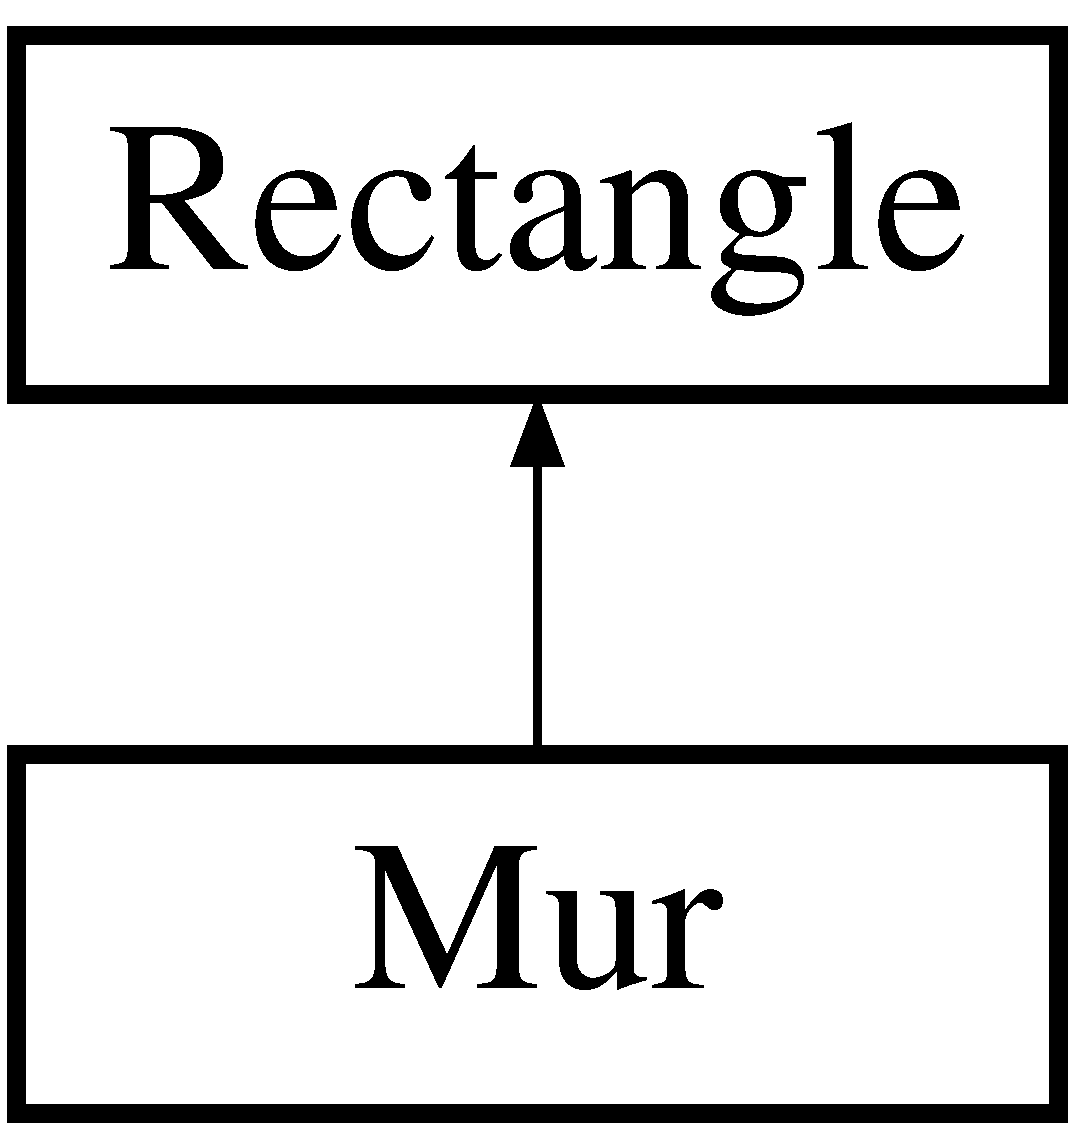
\includegraphics[height=2.000000cm]{class_mur}
\end{center}
\end{figure}
\subsection*{Fonctions membres publiques}
\begin{DoxyCompactItemize}
\item 
\mbox{\hyperlink{class_mur_a52a18f3a0baad70fb413f39e3d29c5a3}{Mur}} (const Vec2 \&\+\_\+pos\+Min=Vec2(0, 0), unsigned int w=1, unsigned int h=1)
\begin{DoxyCompactList}\small\item\em retoune un entier pour dire dans quelle coté la coiilison a lieu et mets la distance dans d \end{DoxyCompactList}\item 
\mbox{\Hypertarget{class_mur_ac17cde341fa126c26a24128d094557a4}\label{class_mur_ac17cde341fa126c26a24128d094557a4}} 
\mbox{\hyperlink{class_mur_ac17cde341fa126c26a24128d094557a4}{Mur}} (const \mbox{\hyperlink{class_rectangle}{Rectangle}} \&r)
\begin{DoxyCompactList}\small\item\em prend un \mbox{\hyperlink{class_rectangle}{Rectangle}} un paramètre pour construire le \mbox{\hyperlink{class_mur}{Mur}} \end{DoxyCompactList}\item 
void \mbox{\hyperlink{class_mur_a63a7560c521670716cd90c3599abcd71}{collision}} (\mbox{\hyperlink{class_cercle}{Cercle}} \&) const
\begin{DoxyCompactList}\small\item\em detecte la collision d\textquotesingle{}un cercle en generale et prend l\textquotesingle{}action necessaire. l\textquotesingle{}action par default est d\textquotesingle{}arrêter le cercle car c\textquotesingle{}est un mur. \end{DoxyCompactList}\item 
\mbox{\hyperlink{class_mur}{Mur}} \mbox{\hyperlink{class_mur_aeb65d73f7f7176a5e77e220107a4902f}{genere\+Mur\+Alea}} (const Vec2 \&, unsigned int w, unsigned int h) const
\begin{DoxyCompactList}\small\item\em retourne le lien vers l\textquotesingle{}image \end{DoxyCompactList}\end{DoxyCompactItemize}
\subsection*{Membres hérités additionnels}


\subsection{Documentation des constructeurs et destructeur}
\mbox{\Hypertarget{class_mur_a52a18f3a0baad70fb413f39e3d29c5a3}\label{class_mur_a52a18f3a0baad70fb413f39e3d29c5a3}} 
\index{Mur@{Mur}!Mur@{Mur}}
\index{Mur@{Mur}!Mur@{Mur}}
\subsubsection{\texorpdfstring{Mur()}{Mur()}}
{\footnotesize\ttfamily Mur\+::\+Mur (\begin{DoxyParamCaption}\item[{const Vec2 \&}]{\+\_\+pos\+Min = {\ttfamily Vec2(0,0)},  }\item[{unsigned int}]{w = {\ttfamily 1},  }\item[{unsigned int}]{h = {\ttfamily 1} }\end{DoxyParamCaption})\hspace{0.3cm}{\ttfamily [inline]}}



retoune un entier pour dire dans quelle coté la coiilison a lieu et mets la distance dans d 

0 pour cote gauche-\/haut 1 pour cote gauche ainsi de suite. donc on tourne dans le snse anti-\/horaire et il y a 8 cote constructeur prend une posotion la largeur et l\textquotesingle{}hauteur en paramètre et au final utilise le constructeur le \mbox{\hyperlink{class_rectangle}{Rectangle}} 

\subsection{Documentation des fonctions membres}
\mbox{\Hypertarget{class_mur_a63a7560c521670716cd90c3599abcd71}\label{class_mur_a63a7560c521670716cd90c3599abcd71}} 
\index{Mur@{Mur}!collision@{collision}}
\index{collision@{collision}!Mur@{Mur}}
\subsubsection{\texorpdfstring{collision()}{collision()}}
{\footnotesize\ttfamily void Mur\+::collision (\begin{DoxyParamCaption}\item[{\mbox{\hyperlink{class_cercle}{Cercle}} \&}]{c }\end{DoxyParamCaption}) const}



detecte la collision d\textquotesingle{}un cercle en generale et prend l\textquotesingle{}action necessaire. l\textquotesingle{}action par default est d\textquotesingle{}arrêter le cercle car c\textquotesingle{}est un mur. 

\begin{DoxyRefDesc}{Bogue}
\item[\mbox{\hyperlink{bug__bug000001}{Bogue}}]des fois la double collision ne marche pas. la plupart des cas c\textquotesingle{}est se voit quand la distance entre deux mur est plus grand que le rayon et inférieur 2$\ast$r.\end{DoxyRefDesc}
\mbox{\Hypertarget{class_mur_aeb65d73f7f7176a5e77e220107a4902f}\label{class_mur_aeb65d73f7f7176a5e77e220107a4902f}} 
\index{Mur@{Mur}!genere\+Mur\+Alea@{genere\+Mur\+Alea}}
\index{genere\+Mur\+Alea@{genere\+Mur\+Alea}!Mur@{Mur}}
\subsubsection{\texorpdfstring{genere\+Mur\+Alea()}{genereMurAlea()}}
{\footnotesize\ttfamily \mbox{\hyperlink{class_mur}{Mur}} Mur\+::genere\+Mur\+Alea (\begin{DoxyParamCaption}\item[{const Vec2 \&}]{pos,  }\item[{unsigned int}]{w,  }\item[{unsigned int}]{h }\end{DoxyParamCaption}) const}



retourne le lien vers l\textquotesingle{}image 

met à jour le lien de l\textquotesingle{}image genere un mur aléatoirement dans le ractangle passe en param 

La documentation de cette classe a été générée à partir des fichiers suivants \+:\begin{DoxyCompactItemize}
\item 
src/core/Mur.\+h\item 
src/core/Mur.\+cpp\end{DoxyCompactItemize}

\hypertarget{class_rectangle}{}\section{Référence de la classe Rectangle}
\label{class_rectangle}\index{Rectangle@{Rectangle}}
Graphe d\textquotesingle{}héritage de Rectangle\+:\begin{figure}[H]
\begin{center}
\leavevmode
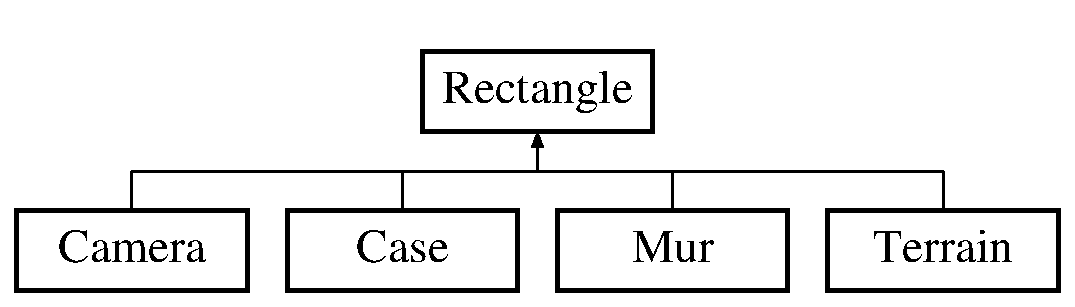
\includegraphics[height=2.000000cm]{class_rectangle}
\end{center}
\end{figure}
\subsection*{Fonctions membres publiques}
\begin{DoxyCompactItemize}
\item 
\mbox{\Hypertarget{class_rectangle_a4f1cd06cacbf4044d1d8cf500c230750}\label{class_rectangle_a4f1cd06cacbf4044d1d8cf500c230750}} 
\mbox{\hyperlink{class_rectangle_a4f1cd06cacbf4044d1d8cf500c230750}{Rectangle}} (const Vec2 \&\+\_\+pos\+Min=Vec2(0, 0), unsigned int w=1, unsigned int h=1)
\begin{DoxyCompactList}\small\item\em cree un rectangle avec \+\_\+pos\+Min comme pos et largeur w et hauteur h \end{DoxyCompactList}\item 
\mbox{\Hypertarget{class_rectangle_a4689a7041fef3b935a2c5e9129f9dfb5}\label{class_rectangle_a4689a7041fef3b935a2c5e9129f9dfb5}} 
\mbox{\hyperlink{class_rectangle_a4689a7041fef3b935a2c5e9129f9dfb5}{Rectangle}} (const \mbox{\hyperlink{class_rectangle}{Rectangle}} \&rec)
\begin{DoxyCompactList}\small\item\em constructeur par copie \end{DoxyCompactList}\item 
\mbox{\Hypertarget{class_rectangle_a494c076b13aadf26efdce07d23c61ddd}\label{class_rectangle_a494c076b13aadf26efdce07d23c61ddd}} 
\mbox{\hyperlink{class_rectangle_a494c076b13aadf26efdce07d23c61ddd}{$\sim$\+Rectangle}} ()
\begin{DoxyCompactList}\small\item\em par default \end{DoxyCompactList}\item 
\mbox{\Hypertarget{class_rectangle_af9782cc2a5f34744beda1443efcddccc}\label{class_rectangle_af9782cc2a5f34744beda1443efcddccc}} 
Vec2 \mbox{\hyperlink{class_rectangle_af9782cc2a5f34744beda1443efcddccc}{get\+Pos}} () const
\begin{DoxyCompactList}\small\item\em get/set pour la position max et min \end{DoxyCompactList}\item 
\mbox{\Hypertarget{class_rectangle_a91792d1be723462563766efd4bb382de}\label{class_rectangle_a91792d1be723462563766efd4bb382de}} 
void {\bfseries set\+Pos} (const Vec2 \&pos)
\item 
\mbox{\Hypertarget{class_rectangle_abd59609e7c494d57f74b1ee46df33f80}\label{class_rectangle_abd59609e7c494d57f74b1ee46df33f80}} 
unsigned int {\bfseries get\+Width} () const
\item 
\mbox{\Hypertarget{class_rectangle_a5bfb002e7628599a47ad4fad1b4fd3c1}\label{class_rectangle_a5bfb002e7628599a47ad4fad1b4fd3c1}} 
unsigned int {\bfseries get\+Height} () const
\item 
\mbox{\Hypertarget{class_rectangle_a65135fe30f29ad6893695e13cee0658c}\label{class_rectangle_a65135fe30f29ad6893695e13cee0658c}} 
void {\bfseries set\+Width} (unsigned int)
\item 
\mbox{\Hypertarget{class_rectangle_aa293da261bdf9580f80c349c772648b1}\label{class_rectangle_aa293da261bdf9580f80c349c772648b1}} 
void {\bfseries set\+Height} (unsigned int)
\item 
\mbox{\Hypertarget{class_rectangle_ae8bf56fea5536645968d0e66aa8da2b7}\label{class_rectangle_ae8bf56fea5536645968d0e66aa8da2b7}} 
bool \mbox{\hyperlink{class_rectangle_ae8bf56fea5536645968d0e66aa8da2b7}{est\+Dans}} (const \mbox{\hyperlink{class_cercle}{Cercle}} \&c) const
\begin{DoxyCompactList}\small\item\em verifie si un cercle est dans un rectangle \end{DoxyCompactList}\item 
\mbox{\Hypertarget{class_rectangle_a8e790c85174f9706bbb4be5255a98e42}\label{class_rectangle_a8e790c85174f9706bbb4be5255a98e42}} 
void \mbox{\hyperlink{class_rectangle_a8e790c85174f9706bbb4be5255a98e42}{sauver}} (int fd) const
\begin{DoxyCompactList}\small\item\em enregistrer le terrain dans un file descripteur. le format est \char`\"{}pos.\+x\textquotesingle{} \textquotesingle{}pos.\+y\textquotesingle{} \textquotesingle{}w\textquotesingle{} \textquotesingle{}h\textquotesingle{}\textbackslash{}n\textquotesingle{}\char`\"{} \end{DoxyCompactList}\item 
\mbox{\Hypertarget{class_rectangle_ae4e6d7f9ff84af1a7c11b62bff7c31b5}\label{class_rectangle_ae4e6d7f9ff84af1a7c11b62bff7c31b5}} 
void \mbox{\hyperlink{class_rectangle_ae4e6d7f9ff84af1a7c11b62bff7c31b5}{charger}} (int fd)
\begin{DoxyCompactList}\small\item\em charge le terrain à d\textquotesingle{}un file descripteur \end{DoxyCompactList}\end{DoxyCompactItemize}
\subsection*{Attributs protégés}
\begin{DoxyCompactItemize}
\item 
\mbox{\Hypertarget{class_rectangle_a77b408f42c985329c92cf4017c0cccbf}\label{class_rectangle_a77b408f42c985329c92cf4017c0cccbf}} 
Vec2 {\bfseries pos}
\item 
\mbox{\Hypertarget{class_rectangle_acd28f1ca4b37a5563ca04900a04e6a61}\label{class_rectangle_acd28f1ca4b37a5563ca04900a04e6a61}} 
unsigned int {\bfseries w}
\item 
\mbox{\Hypertarget{class_rectangle_a1f6826771367cf8bbc891002879af25a}\label{class_rectangle_a1f6826771367cf8bbc891002879af25a}} 
unsigned int {\bfseries h}
\end{DoxyCompactItemize}
\subsection*{Amis}
\begin{DoxyCompactItemize}
\item 
\mbox{\Hypertarget{class_rectangle_a4ad36cfac2439cc552d60271d657b756}\label{class_rectangle_a4ad36cfac2439cc552d60271d657b756}} 
std\+::ostream \& \mbox{\hyperlink{class_rectangle_a4ad36cfac2439cc552d60271d657b756}{operator$<$$<$}} (std\+::ostream \&flux, const \mbox{\hyperlink{class_rectangle}{Rectangle}} \&r)
\begin{DoxyCompactList}\small\item\em surcharge pour des flux de sortie comme cout$<$$<$ \end{DoxyCompactList}\item 
\mbox{\Hypertarget{class_rectangle_ac8aa7e7afae9a4ff96c594710019e9f5}\label{class_rectangle_ac8aa7e7afae9a4ff96c594710019e9f5}} 
std\+::istream \& \mbox{\hyperlink{class_rectangle_ac8aa7e7afae9a4ff96c594710019e9f5}{operator$>$$>$}} (std\+::istream \&flux, \mbox{\hyperlink{class_rectangle}{Rectangle}} \&r)
\begin{DoxyCompactList}\small\item\em surcharge pour des fllux d\textquotesingle{}entrée comme cin$>$$>$ \end{DoxyCompactList}\end{DoxyCompactItemize}


La documentation de cette classe a été générée à partir des fichiers suivants \+:\begin{DoxyCompactItemize}
\item 
src/base/Rectangle.\+h\item 
src/base/Rectangle.\+cpp\end{DoxyCompactItemize}

\hypertarget{class_reseau}{}\section{Référence de la classe Reseau}
\label{class_reseau}\index{Reseau@{Reseau}}
\subsection*{Fonctions membres publiques}
\begin{DoxyCompactItemize}
\item 
\mbox{\Hypertarget{class_reseau_a89620a20271951433e894005be3841b4}\label{class_reseau_a89620a20271951433e894005be3841b4}} 
void {\bfseries init} ()
\item 
\mbox{\Hypertarget{class_reseau_a60d37f0cbdfc9612c47cd3764a109533}\label{class_reseau_a60d37f0cbdfc9612c47cd3764a109533}} 
int {\bfseries get\+\_\+connection} () const
\item 
\mbox{\Hypertarget{class_reseau_a28eb685fc185d8bcbfcb3cc23b97ef91}\label{class_reseau_a28eb685fc185d8bcbfcb3cc23b97ef91}} 
bool {\bfseries is\+\_\+server} () const
\item 
\mbox{\Hypertarget{class_reseau_ae8a8c3dbcfd6c771c5b7bd13079eb2e6}\label{class_reseau_ae8a8c3dbcfd6c771c5b7bd13079eb2e6}} 
bool {\bfseries flip\+\_\+trun} ()
\end{DoxyCompactItemize}
\subsection*{Fonctions membres protégées}
\begin{DoxyCompactItemize}
\item 
\mbox{\Hypertarget{class_reseau_a01be2a7060fb903f92386ab8b37d985e}\label{class_reseau_a01be2a7060fb903f92386ab8b37d985e}} 
bool \mbox{\hyperlink{class_reseau_a01be2a7060fb903f92386ab8b37d985e}{valid\+\_\+ip}} (const std\+::string \&ip)
\begin{DoxyCompactList}\small\item\em vérifie la validité d\textquotesingle{}une adresse ip . \end{DoxyCompactList}\end{DoxyCompactItemize}
\subsection*{Attributs protégés}
\begin{DoxyCompactItemize}
\item 
\mbox{\Hypertarget{class_reseau_a92d4e0d43960bdf0b224c2de7c040e26}\label{class_reseau_a92d4e0d43960bdf0b224c2de7c040e26}} 
int {\bfseries connection}
\item 
\mbox{\Hypertarget{class_reseau_a06285e1858413fbf99fbffa973393018}\label{class_reseau_a06285e1858413fbf99fbffa973393018}} 
bool {\bfseries v\+\_\+is\+\_\+server}
\item 
\mbox{\Hypertarget{class_reseau_a6e6d0830e491ed7b7ccb0205258a0ab7}\label{class_reseau_a6e6d0830e491ed7b7ccb0205258a0ab7}} 
bool {\bfseries v\+\_\+flip\+\_\+turn}
\end{DoxyCompactItemize}


La documentation de cette classe a été générée à partir des fichiers suivants \+:\begin{DoxyCompactItemize}
\item 
src/base/Reseau.\+h\item 
src/base/Reseau.\+cpp\end{DoxyCompactItemize}

\hypertarget{class_tab_dyn}{}\section{Référence du modèle de la classe Tab\+Dyn$<$ T $>$}
\label{class_tab_dyn}\index{Tab\+Dyn$<$ T $>$@{Tab\+Dyn$<$ T $>$}}
\subsection*{Fonctions membres publiques}
\begin{DoxyCompactItemize}
\item 
\mbox{\Hypertarget{class_tab_dyn_a24d80afe7593c82ec106d43684a2d188}\label{class_tab_dyn_a24d80afe7593c82ec106d43684a2d188}} 
T {\bfseries elementI} (unsigned int indice) const
\item 
\mbox{\Hypertarget{class_tab_dyn_a30c1fe4f663161624e1138821c847b90}\label{class_tab_dyn_a30c1fe4f663161624e1138821c847b90}} 
void {\bfseries ajouter\+Element} (const T \&)
\item 
\mbox{\Hypertarget{class_tab_dyn_a61cd5aeb1186bd7e37d5777e2d24e9e3}\label{class_tab_dyn_a61cd5aeb1186bd7e37d5777e2d24e9e3}} 
unsigned int {\bfseries taille\+\_\+utilise} () const
\item 
\mbox{\Hypertarget{class_tab_dyn_a554b655e742b69653de45da760941474}\label{class_tab_dyn_a554b655e742b69653de45da760941474}} 
void {\bfseries trier} ()
\item 
\mbox{\Hypertarget{class_tab_dyn_a0bc6df9417462c573617d6b09a048426}\label{class_tab_dyn_a0bc6df9417462c573617d6b09a048426}} 
void {\bfseries supprimer\+ElementI} (unsigned int indice)
\item 
\mbox{\Hypertarget{class_tab_dyn_a383e37b33119227258564ccd052ffe74}\label{class_tab_dyn_a383e37b33119227258564ccd052ffe74}} 
void {\bfseries afficher\+Tab} () const
\item 
\mbox{\Hypertarget{class_tab_dyn_ad76fed652f27c5833c78db659abc291c}\label{class_tab_dyn_ad76fed652f27c5833c78db659abc291c}} 
void \mbox{\hyperlink{class_tab_dyn_ad76fed652f27c5833c78db659abc291c}{sauver\+Tab}} (const std\+::string \&chemin)
\begin{DoxyCompactList}\small\item\em sauvgarde le tableau en vidant le ficher dans le ficher passé en parametre \end{DoxyCompactList}\item 
\mbox{\Hypertarget{class_tab_dyn_a0691ddc682fa501ce7dbd0a7d1f9e261}\label{class_tab_dyn_a0691ddc682fa501ce7dbd0a7d1f9e261}} 
void \mbox{\hyperlink{class_tab_dyn_a0691ddc682fa501ce7dbd0a7d1f9e261}{charger\+Tab}} (const std\+::string \&chemin)
\begin{DoxyCompactList}\small\item\em charge le tableau à partir du ficher. \end{DoxyCompactList}\item 
void \mbox{\hyperlink{class_tab_dyn_acfc88ef40cb66400e9dd2ff120b5273a}{sauver\+Tab}} (int fd)
\begin{DoxyCompactList}\small\item\em sauvgarde le tableau dans le descripteur du ficher. \end{DoxyCompactList}\item 
void \mbox{\hyperlink{class_tab_dyn_acd5db90f6eb28d32314e91586d43b1a3}{charger\+Tab}} (int fd)
\begin{DoxyCompactList}\small\item\em charge le tableau à partir du descripteur du ficher. \end{DoxyCompactList}\end{DoxyCompactItemize}
\subsection*{Attributs protégés}
\begin{DoxyCompactItemize}
\item 
\mbox{\Hypertarget{class_tab_dyn_a5cc36063858ffd2fabb9b87aa04ae10b}\label{class_tab_dyn_a5cc36063858ffd2fabb9b87aa04ae10b}} 
std\+::vector$<$ T $>$ {\bfseries elements}
\end{DoxyCompactItemize}


\subsection{Documentation des fonctions membres}
\mbox{\Hypertarget{class_tab_dyn_acd5db90f6eb28d32314e91586d43b1a3}\label{class_tab_dyn_acd5db90f6eb28d32314e91586d43b1a3}} 
\index{Tab\+Dyn@{Tab\+Dyn}!charger\+Tab@{charger\+Tab}}
\index{charger\+Tab@{charger\+Tab}!Tab\+Dyn@{Tab\+Dyn}}
\subsubsection{\texorpdfstring{charger\+Tab()}{chargerTab()}}
{\footnotesize\ttfamily template$<$class T $>$ \\
void \mbox{\hyperlink{class_tab_dyn}{Tab\+Dyn}}$<$ T $>$\+::charger\+Tab (\begin{DoxyParamCaption}\item[{int}]{fd }\end{DoxyParamCaption})}



charge le tableau à partir du descripteur du ficher. 


\begin{DoxyParams}{Paramètres}
{\em le} & descripteur du ficher peut être un socket ou pipe \\
\hline
\end{DoxyParams}
\mbox{\Hypertarget{class_tab_dyn_acfc88ef40cb66400e9dd2ff120b5273a}\label{class_tab_dyn_acfc88ef40cb66400e9dd2ff120b5273a}} 
\index{Tab\+Dyn@{Tab\+Dyn}!sauver\+Tab@{sauver\+Tab}}
\index{sauver\+Tab@{sauver\+Tab}!Tab\+Dyn@{Tab\+Dyn}}
\subsubsection{\texorpdfstring{sauver\+Tab()}{sauverTab()}}
{\footnotesize\ttfamily template$<$class T $>$ \\
void \mbox{\hyperlink{class_tab_dyn}{Tab\+Dyn}}$<$ T $>$\+::sauver\+Tab (\begin{DoxyParamCaption}\item[{int}]{fd }\end{DoxyParamCaption})}



sauvgarde le tableau dans le descripteur du ficher. 


\begin{DoxyParams}{Paramètres}
{\em le} & descripteur du ficher peut être un socket ou pipe \\
\hline
\end{DoxyParams}


La documentation de cette classe a été générée à partir du fichier suivant \+:\begin{DoxyCompactItemize}
\item 
src/base/Tab\+Dyn.\+h\end{DoxyCompactItemize}

\hypertarget{class_terrain}{}\section{Référence de la classe Terrain}
\label{class_terrain}\index{Terrain@{Terrain}}


un terrain possède une position, un largeur et une hauteur.  




{\ttfamily \#include $<$Terrain.\+h$>$}

Graphe d\textquotesingle{}héritage de Terrain\+:\begin{figure}[H]
\begin{center}
\leavevmode
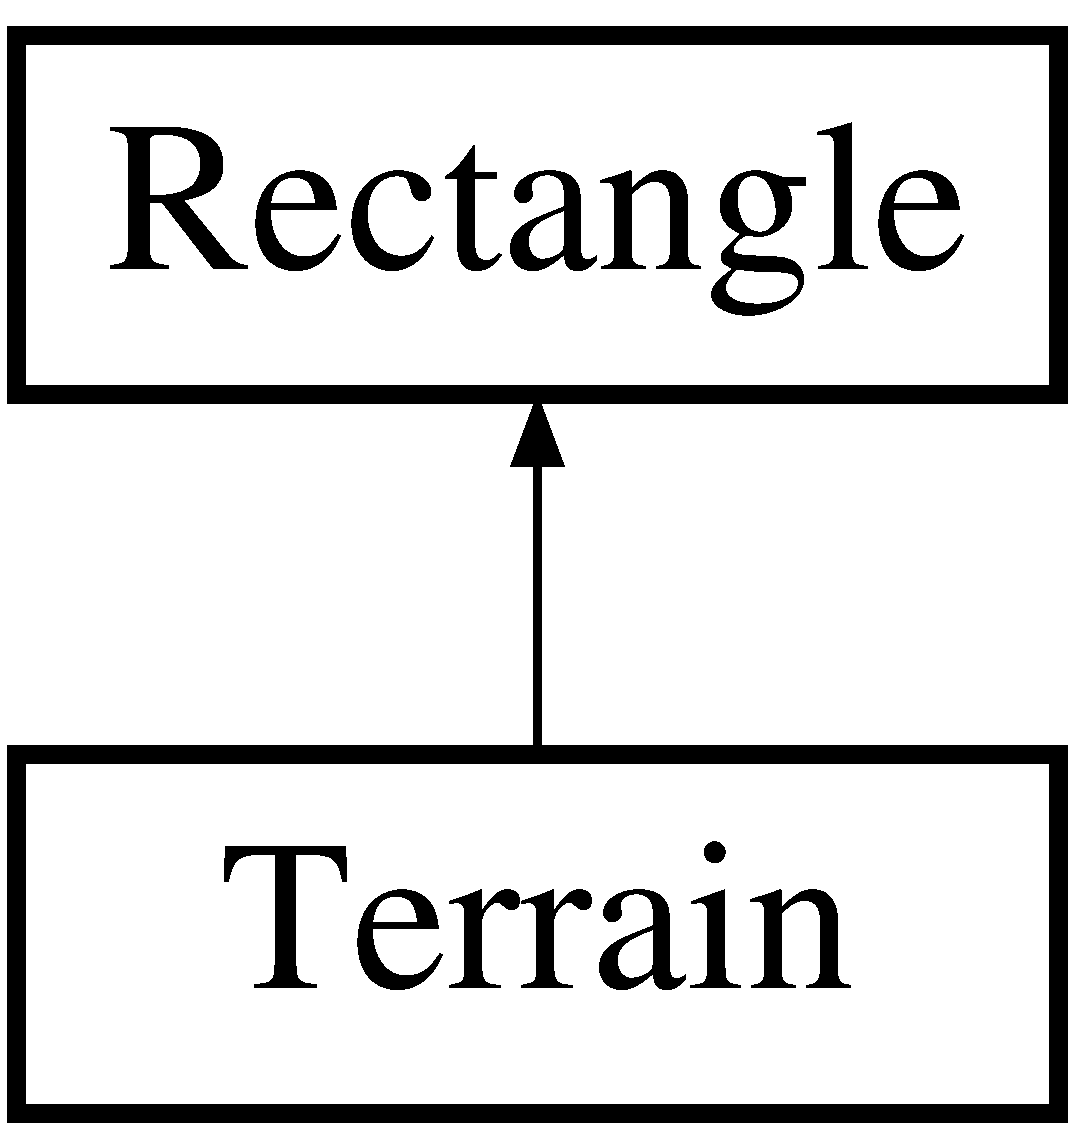
\includegraphics[height=2.000000cm]{class_terrain}
\end{center}
\end{figure}
\subsection*{Fonctions membres publiques}
\begin{DoxyCompactItemize}
\item 
\mbox{\Hypertarget{class_terrain_a3b01a8d47de9ad7b913236c1ab9f62ce}\label{class_terrain_a3b01a8d47de9ad7b913236c1ab9f62ce}} 
\mbox{\hyperlink{class_terrain_a3b01a8d47de9ad7b913236c1ab9f62ce}{Terrain}} (const Vec2 \&\+\_\+pos\+Min=Vec2(0, 0), unsigned int w=1, unsigned int h=1)
\begin{DoxyCompactList}\small\item\em Constructeur par default utilise celle du \mbox{\hyperlink{class_rectangle}{Rectangle}}. \end{DoxyCompactList}\item 
\mbox{\Hypertarget{class_terrain_a193cb653a018575760d02e2819cb550c}\label{class_terrain_a193cb653a018575760d02e2819cb550c}} 
{\bfseries Terrain} (const \mbox{\hyperlink{class_rectangle}{Rectangle}} \&rec)
\item 
void \mbox{\hyperlink{class_terrain_a9546059cb210f4e4f90905ba9d0f23ea}{collision}} (\mbox{\hyperlink{class_cercle}{Cercle}} \&) const
\begin{DoxyCompactList}\small\item\em verifie si le cercle sort du terrain dans le cercle sort il le remet dans le terrain \end{DoxyCompactList}\item 
\mbox{\Hypertarget{class_terrain_a981fe71718eaa146e0b8fe7bb771b38c}\label{class_terrain_a981fe71718eaa146e0b8fe7bb771b38c}} 
void \mbox{\hyperlink{class_terrain_a981fe71718eaa146e0b8fe7bb771b38c}{collision}} (\mbox{\hyperlink{class_rectangle}{Rectangle}} \&)
\begin{DoxyCompactList}\small\item\em verifie si le \mbox{\hyperlink{class_rectangle}{Rectangle}} sort du terrain dans le cercle sort il le remet dans le terrain \end{DoxyCompactList}\end{DoxyCompactItemize}
\subsection*{Membres hérités additionnels}


\subsection{Description détaillée}
un terrain possède une position, un largeur et une hauteur. 

les accesseur et les mutateur sont les meme que le class \mbox{\hyperlink{class_rectangle}{Rectangle}}. en plus des focntions de la classe \mbox{\hyperlink{class_rectangle}{Rectangle}} le terrain dectect ausssi les cillisions et ainsi ne permet pas aux objets de sortir du terrain 

\subsection{Documentation des fonctions membres}
\mbox{\Hypertarget{class_terrain_a9546059cb210f4e4f90905ba9d0f23ea}\label{class_terrain_a9546059cb210f4e4f90905ba9d0f23ea}} 
\index{Terrain@{Terrain}!collision@{collision}}
\index{collision@{collision}!Terrain@{Terrain}}
\subsubsection{\texorpdfstring{collision()}{collision()}}
{\footnotesize\ttfamily void Terrain\+::collision (\begin{DoxyParamCaption}\item[{\mbox{\hyperlink{class_cercle}{Cercle}} \&}]{c }\end{DoxyParamCaption}) const}



verifie si le cercle sort du terrain dans le cercle sort il le remet dans le terrain 

empeche la sortie du terrain en replaçant l\textquotesingle{}objet à sa posiotion precedente . 

La documentation de cette classe a été générée à partir des fichiers suivants \+:\begin{DoxyCompactItemize}
\item 
src/core/Terrain.\+h\item 
src/core/Terrain.\+cpp\end{DoxyCompactItemize}

\chapter{Documentation des fichiers}
\hypertarget{socklib_8hpp}{}\section{Référence du fichier src/base/socklib.hpp}
\label{socklib_8hpp}\index{src/base/socklib.\+hpp@{src/base/socklib.\+hpp}}


fichier contenant les fonctions de créations de socket et les fonctions de gestion d\textquotesingle{}erreur  


{\ttfamily \#include $<$cerrno$>$}\newline
{\ttfamily \#include $<$string$>$}\newline
\subsection*{Espaces de nommage}
\begin{DoxyCompactItemize}
\item 
 \mbox{\hyperlink{namespacesocklib}{socklib}}
\begin{DoxyCompactList}\small\item\em espace de nom général \end{DoxyCompactList}\end{DoxyCompactItemize}
\subsection*{Macros}
\begin{DoxyCompactItemize}
\item 
\#define \mbox{\hyperlink{socklib_8hpp_a1453d82227a8342fea2b5cf8f8d74dbc}{exit\+\_\+error}}(msg,  cond,  errnum)~\mbox{\hyperlink{namespacesocklib_aec23e1a0b60ca039283516d2305f799e}{socklib\+::\+\_\+\+\_\+error\+\_\+}}(\+\_\+\+\_\+\+F\+I\+L\+E\+\_\+\+\_\+, \+\_\+\+\_\+\+L\+I\+N\+E\+\_\+\+\_\+, (msg), cond, errnum, true)
\begin{DoxyCompactList}\small\item\em fonction de test et de génération d\textquotesingle{}erreur \end{DoxyCompactList}\item 
\#define \mbox{\hyperlink{socklib_8hpp_a8bcb357083c8c3b9443156cf9ed2dc82}{warning\+\_\+error}}(msg,  cond,  errnum)~\mbox{\hyperlink{namespacesocklib_aec23e1a0b60ca039283516d2305f799e}{socklib\+::\+\_\+\+\_\+error\+\_\+}}(\+\_\+\+\_\+\+F\+I\+L\+E\+\_\+\+\_\+, \+\_\+\+\_\+\+L\+I\+N\+E\+\_\+\+\_\+, (msg), cond, errnum, false)
\begin{DoxyCompactList}\small\item\em fonction de test provoquant un warning \end{DoxyCompactList}\end{DoxyCompactItemize}
\subsection*{Fonctions}
\begin{DoxyCompactItemize}
\item 
void \mbox{\hyperlink{namespacesocklib_aec23e1a0b60ca039283516d2305f799e}{socklib\+::\+\_\+\+\_\+error\+\_\+}} (const char $\ast$file, const int ligne, const std\+::string \&msg, bool cond, int errnum, bool exception)
\begin{DoxyCompactList}\small\item\em fonction générique de la gestion d\textquotesingle{}erreur \end{DoxyCompactList}\item 
int \mbox{\hyperlink{namespacesocklib_af229dcfe18deb451a8163a02ea5a3b06}{socklib\+::\+Cree\+Socket\+Serveur}} (const std\+::string \&port)
\begin{DoxyCompactList}\small\item\em Cree une socket d\textquotesingle{}attente pour le serveur sur le port \textquotesingle{}\textquotesingle{}port\textquotesingle{}\textquotesingle{}. \end{DoxyCompactList}\item 
int \mbox{\hyperlink{namespacesocklib_a426a4d6e2fbcf559659e88607f0473f7}{socklib\+::\+Cree\+Socket\+Client}} (const std\+::string \&server, const std\+::string \&port)
\begin{DoxyCompactList}\small\item\em Crée une socket de client en se connectant à un serveur. \end{DoxyCompactList}\item 
int \mbox{\hyperlink{namespacesocklib_a56cdbced316496706a18df3f6a62d28f}{socklib\+::\+Accept\+Connexion}} (int s)
\begin{DoxyCompactList}\small\item\em Accepte un nouveau client. \end{DoxyCompactList}\end{DoxyCompactItemize}


\subsection{Description détaillée}
fichier contenant les fonctions de créations de socket et les fonctions de gestion d\textquotesingle{}erreur 



\subsection{Documentation des macros}
\mbox{\Hypertarget{socklib_8hpp_a1453d82227a8342fea2b5cf8f8d74dbc}\label{socklib_8hpp_a1453d82227a8342fea2b5cf8f8d74dbc}} 
\index{socklib.\+hpp@{socklib.\+hpp}!exit\+\_\+error@{exit\+\_\+error}}
\index{exit\+\_\+error@{exit\+\_\+error}!socklib.\+hpp@{socklib.\+hpp}}
\subsubsection{\texorpdfstring{exit\+\_\+error}{exit\_error}}
{\footnotesize\ttfamily \#define exit\+\_\+error(\begin{DoxyParamCaption}\item[{}]{msg,  }\item[{}]{cond,  }\item[{}]{errnum }\end{DoxyParamCaption})~\mbox{\hyperlink{namespacesocklib_aec23e1a0b60ca039283516d2305f799e}{socklib\+::\+\_\+\+\_\+error\+\_\+}}(\+\_\+\+\_\+\+F\+I\+L\+E\+\_\+\+\_\+, \+\_\+\+\_\+\+L\+I\+N\+E\+\_\+\+\_\+, (msg), cond, errnum, true)}



fonction de test et de génération d\textquotesingle{}erreur 


\begin{DoxyParams}{Paramètres}
{\em msg} & \+: message à afficher \\
\hline
{\em cond} & \+: condition d\textquotesingle{}erreur \\
\hline
{\em errnum} & \+: numéro de l\textquotesingle{}erreur système ou 0 s\textquotesingle{}il n\textquotesingle{}y en a pas.\\
\hline
\end{DoxyParams}
Cette fonction affiche le texte d\textquotesingle{}erreur {\ttfamily msg} sur la sortie d\textquotesingle{}erreur et lance une exception. Si un code d\textquotesingle{}erreur {\ttfamily errnum} différent de 0 est fourni, l\textquotesingle{}exception générée est une erreur système (std\+::system\+\_\+error) dont {\ttfamily errnum} est le code d\textquotesingle{}erreur. Sinon, l\textquotesingle{}exception est une std\+::runtime\+\_\+error dont {\ttfamily msg} est le message.

Par exemple le code suivant ouvre un FD en écriture en créant le fichier {\ttfamily toto.\+txt} et teste sa création et génère une exception système en cas d\textquotesingle{}erreur 
\begin{DoxyCode}
fdout = open(\textcolor{stringliteral}{"toto.txt"}, O\_CREAT|O\_WRONLY, S\_IRUSR|S\_IWUSR);
\mbox{\hyperlink{socklib_8hpp_a1453d82227a8342fea2b5cf8f8d74dbc}{exit\_error}}(\textcolor{stringliteral}{"Création du fichier"}, fdout==-1, errno);
\end{DoxyCode}
 \mbox{\Hypertarget{socklib_8hpp_a8bcb357083c8c3b9443156cf9ed2dc82}\label{socklib_8hpp_a8bcb357083c8c3b9443156cf9ed2dc82}} 
\index{socklib.\+hpp@{socklib.\+hpp}!warning\+\_\+error@{warning\+\_\+error}}
\index{warning\+\_\+error@{warning\+\_\+error}!socklib.\+hpp@{socklib.\+hpp}}
\subsubsection{\texorpdfstring{warning\+\_\+error}{warning\_error}}
{\footnotesize\ttfamily \#define warning\+\_\+error(\begin{DoxyParamCaption}\item[{}]{msg,  }\item[{}]{cond,  }\item[{}]{errnum }\end{DoxyParamCaption})~\mbox{\hyperlink{namespacesocklib_aec23e1a0b60ca039283516d2305f799e}{socklib\+::\+\_\+\+\_\+error\+\_\+}}(\+\_\+\+\_\+\+F\+I\+L\+E\+\_\+\+\_\+, \+\_\+\+\_\+\+L\+I\+N\+E\+\_\+\+\_\+, (msg), cond, errnum, false)}



fonction de test provoquant un warning 


\begin{DoxyParams}{Paramètres}
{\em msg} & \+: message à afficher \\
\hline
{\em cond} & \+: condition d\textquotesingle{}erreur \\
\hline
{\em errnum} & \+: numéro de l\textquotesingle{}erreur système ou 0 s\textquotesingle{}il n\textquotesingle{}y en a pas.\\
\hline
\end{DoxyParams}
teste la condition cond et affiche un warning.

Cette fonction affiche le texte d\textquotesingle{}erreur {\ttfamily msg} sur la sortie d\textquotesingle{}erreur. Si un code d\textquotesingle{}erreur {\ttfamily errnum} différent de 0 est fourni, l\textquotesingle{}exception générée est une erreur système (std\+::system\+\_\+error) dont {\ttfamily errnum} est le code d\textquotesingle{}erreur. Sinon, l\textquotesingle{}execption est une std\+::runtime\+\_\+error dont {\ttfamily msg} est le message. 
%--- End generated contents ---

% Index
\backmatter
\newpage
\phantomsection
\clearemptydoublepage
\addcontentsline{toc}{chapter}{Index}
\printindex

\end{document}
